%%%%%%%%%%%%%
%% Results %%
%%%%%%%%%%%%%

\chapter{Results} \label{Ch:Results}
In this chapter, the results for the experiment described in section~\ref{Sec:Experiments} are reported. This includes ablation studies, parameter tests and registration performance assessment on the \emph{ACDC} dataset as well as a motion-compensated reconstruction pipeline on the \emph{CMRxRecon} dataset.
 
\section{Ablation Studies and Parameter Tests} \label{Sec:ResultsParameterTestsACDC}
In this section, the results for the ablation studies and parameter tests are described in section~\ref{SubSec:ParameterTestsACDC} are presented.

\subsection{Fourier-Net versus Fourier-Net+} \label{SubSec:ResultsFourier-NetvsFourier-Net+ACDC}
First, \emph{Fourier-Net}, \emph{Fourier-Net+} and \emph{4xFourier-Net} were compared as described in section~\ref{SubSubSec:Fourier-NetvsFourier-Net+}. The results can be seen in Table~\ref{tab:Fourier-NetvsFourier-Net+ACDC}. For the dense displacement variants, the diffeomorphic transform increases the Dice score (with and without the background label) slightly for \emph{Fourier-Net} and \emph{4xFourier-Net}, but decreases for \emph{Fourier-Net+}. The SSIM decreases for all models slightly, while the MSE remains unaffected. Unsurprisingly, the percentage of non-positive Jabobian determinants is lower for the diffeomorphic variants. Times for the baseline and diffeomorphic versions are similar with the \emph{Fourier-Net} being faster without the diffeomorphism by 1.2~ms, while \emph{Fourier-Net+} and \emph{4xFourier-Net} are faster with the diffeomorphism by 3.2~ms and 1.6~ms respectively. \\
The results for the band-limited versions are very similar with \emph{Fourier-Net} and \emph{Fourier-Net+} having a lower Dice (with background) with the diffeomorphism, while \emph{4xFourier-Net} increases by almost 2$\%$. When excluding the background label \emph{Fourier-Net} is again slightly worse, but \emph{Fourier-Net+} and \emph{4xFourier-Net} both improve, the latter with almost 3$\%$ Dice more than the baseline version. The SSIM values are slightly lower for \emph{Fourier-Net} and \emph{Fourier-Net+} with the diffeomorphism, but again higher for \emph{4xFourier-Net}. The MSE is slightly lower for \emph{Fourier-Net} and \emph{4xFourier-Net}, but slightly higher for \emph{Fourier-Net+}. The percentage of non-positive Jabobian determinants again decreases for the diffeomorphic variants. The times again vary slightly with \emph{Fourier-Net} and \emph{Fourier-Net+} being slower by 0.5~ms and 6.2~ms, while \emph{4xFourier-Net} is a lot faster with 14.7~ms difference.\\
Now to the difference between the dense and band-limited displacement. Overall, the dense displacement versions have a higher Dice score for all models both with and without the background label.  The dense displacements also have better SSIM and MSE metrics, however the difference is not quite as large as with the Dice scores.  Only the percentage of non-positive Jabobian determinants is notably lower for the band-limited displacement. In terms of inference time, the dense displacement variants are slightly faster despite having a larger encoder, however all of the models are in the milliseconds (7~ms up to 33.5~ms). Last but not least, the memory consumption needs to be addressed. The dense displacment variants have a larger encoder, as discussed before, and thus have far more parameters, especially for the more optimized \emph{Fourier-Net+} and \emph{4xFourier-Net} (about 5 times more). The number of Mult-Adds and the amount of total memory are more than doubled (almost tripled for \emph{4xFourier-Net}) for the dense displacement versions compared to those with a band-limited displacement across all models.

\begin{table}[h] %htpb
	%\scriptsize
	\centering
	\caption{Results for the \emph{Fourier-Net versus Fourier-Net+} experiment. The networks are compared using both dense and band-limited displacement fields as well as diffeomorphic transforms on the fully sampled \emph{ACDC} test data.}
	\label{tab:Fourier-NetvsFourier-Net+ACDC}
	\begin{tabularx}{\textwidth}{Y Y Y Y Y} 
		\toprule
		\multirow{2}{*}{Metrics} & \multicolumn{3}{c}{Dense Displacement} \\
		\cmidrule(lr){2-4} 
		 & Fourier-Net & Fourier-Net+ & 4xFourier-Net+\\	
		\midrule
		$\%$ Dice $\uparrow$ & $78.22 \pm 13.84$ & $78.43 \pm 13.96$ & \textbf{79.34} $\pm$ \textbf{14.03}\\
		$\%$ Dice* $\uparrow$ & $71.03 \pm 18.87$ & $70.50 \pm 19.17$ & \textbf{72.02} $\pm$ \textbf{18.94} \\
		$\%$ SSIM $\uparrow$ & \textbf{91.92} $\pm$ \textbf{3.32} & $89.09 \pm 4.10$ & $89.65 \pm 3.85$\\
		MSE (m) $\downarrow$ & \textbf{0.09} $\pm$ \textbf{0.06} & $0.17 \pm 0.13$ & $0.15 \pm 0.12$ \\
		$\% \, |J_{\phi}|\leq0 \downarrow$ & $0.53 \pm 0.52$ & $0.32 \pm 0.55$ & \textbf{0.04} $\pm$ \textbf{0.09} \\
		Time [ms] $\downarrow$  & \textbf{7.03} 	& 10.74 	& 21.89 \\
		\midrule
		 & \mbox{Diff-Fourier-Net} & \mbox{Diff-Fourier-Net+} & \mbox{Diff-4xFourier-Net+}\\		
		\midrule
		$\%$ Dice $\uparrow$ & $78.56 \pm 14.13$ & $77.88 \pm 13.81$ & \textbf{79.49} $\pm$ \textbf{14.26}\\
		$\%$ Dice* $\uparrow$ & $71.31 \pm 19.13$ & $70.19 \pm 18.82$ & \textbf{72.12} $\pm$ \textbf{19.33} \\
		$\%$ SSIM $\uparrow$ & \textbf{91.79} $\pm$ \textbf{3.38} & $89.08 \pm 4.10$ & $89.62 \pm 3.98$\\
		MSE (m) $\downarrow$ & \textbf{0.09} $\pm$ \textbf{0.06} & $0.16 \pm 0.13$ & $0.15 \pm 0.12$ \\
		$\% \, |J_{\phi}|\leq0 \downarrow$ & $0.03 \pm 0.06$ & $0.00 \pm 0.00$ & $0.00 \pm 0.00$ \\
		Time [ms] $\downarrow$  & 8.16  & \textbf{7.46} & 20.33 \\
		\midrule
		Parameters $\downarrow$ & 645,216 & \textbf{380,470} & 1,521,880 \\
		Mult-Adds (G) $\downarrow$ & 1.12  	& \textbf{0.04} 	& 0.18 \\
		Memory [MB] $\downarrow$ & 97.63   & \textbf{5.81} 	& 21.90 \\
		\bottomrule
	\end{tabularx}
\end{table}
% split table to fit better onto the pages
\begin{table}[H]		
	\centering
	\begin{tabularx}{\textwidth}{Y Y Y Y Y}
		\toprule	
		\multirow{2}{*}{Metrics} & \multicolumn{3}{c}{Band-limited Displacement} \\
		\cmidrule(lr){2-4} 
		 & Fourier-Net & Fourier-Net+ & 4xFourier-Net+\\		
		\midrule
		$\%$ Dice $\uparrow$ & \textbf{77.95} $\pm$ \textbf{14.71} & $75.35 \pm 14.28$ & $76.59 \pm 14.84$\\
		$\%$ Dice* $\uparrow$ & \textbf{69.96} $\pm$ \textbf{21.55} & $64.74 \pm 21.12$ & $66.82 \pm 21.55$ \\
		$\%$ SSIM $\uparrow$ & \textbf{91.35} $\pm$ \textbf{3.51} & $88.42 \pm 3.94$ & $88.59 \pm 4.23$\\
		MSE (m) $\downarrow$ & \textbf{1.00} $\pm$ \textbf{0.71} & $2.06 \pm 1.54$ & $1.92 \pm 1.46$ \\
		$\% \, |J_{\phi}|\leq0 \downarrow$ & $0.36 \pm 0.38$ & $0.13 \pm 0.35$ & \textbf{0.03} $\pm$ \textbf{0.12} \\
		Time [ms] $\downarrow$ & \textbf{14.46} & \textbf{14.46} & 33.49 \\
		\midrule
		 & \mbox{Diff-Fourier-Net} & \mbox{Diff-Fourier-Net+} & \mbox{Diff-4xFourier-Net+}\\		
		\midrule
		$\%$ Dice $\uparrow$ & $77.93 \pm 14.93$ & $75.17 \pm 13.43$ & \textbf{78.20} $\pm$ \textbf{14.01}\\
		$\%$ Dice* $\uparrow$ & \textbf{69.91} $\pm$ \textbf{21.99} & $65.67 \pm 18.61$ & $69.61 \pm 19.11$ \\
		$\%$ SSIM $\uparrow$ & \textbf{91.24} $\pm$ \textbf{3.56} & $87.81 \pm 3.94$ & $88.81 \pm 4.13$\\
		MSE (m) $\downarrow$ & \textbf{0.98} $\pm$ \textbf{0.67} & $2.29 \pm 1.61$ & $1.85 \pm 1.41$ \\
		$\% \, |J_{\phi}|\leq0 \downarrow$ & $0.01 \pm 0.03$ & \textbf{0.00} $\pm$ \textbf{0.00} & \textbf{0.00} $\pm$ \textbf{0.00} \\
		Time [ms] $\downarrow$ 	  & \textbf{14.96}  & 20.72 & 18.81 \\
		\midrule
		Parameters $\downarrow$    & 434,519 & \textbf{75,429} & 301,716 \\
		Mult-Adds (M) $\downarrow$ & 595.04  & \textbf{10.98}  & 43.91 \\
		Memory [MB] $\downarrow$   & 44.69   & \textbf{2.25}   & 7.66 \\
		\bottomrule
	\end{tabularx}
\end{table}


\subsection{Starting Channel Size} \label{SubSec:ResultsStartingChannelsACDC}
Next, the impact of the starting channel size was examined as explained in section~\ref{SubSubSec:StartingChannelsACDC}. The results can be seen in Table~\ref{tab:StartingChannelsFourierNet+ACDC}. The Dice (with and without the background label) increased for both \emph{Fourier-Net+} and \emph{4xFourier-Net+} for larger channel sizes. A marginal increase in SSIM and MSE was observed, while the percentage of non-positive Jabobian determinants decreased. The inference time is not heavily impacted by channel size as the times remain very similar for all sizes. The number of parameters drastically increases with starting size leading to an increase in Mult-Add and thus overall memory. As \emph{4xFourier-Net+} is just a cascaded version of \emph{Fourier-Net+} a channel size of 16 for the latter is about the same as channel size~8 for the cascaded version and so on. This can also be seen in the direct comparison between \emph{Fourier-Net+} and \emph{4xFourier-Net+}, where the latter has a better performance, but also needs more memory. While an increase of channel size also increases performance in terms of Dice (with the background label) by $0.36\%$, $0.43\%$ and $0.41\%$ for the latter, which is quite consistent, it can be observed that an increase of channel size for \emph{Fourier-Net+} has an bigger impact at the beginning ($1.38\%$, $0.78\%$ and $0.15\%$) and fades towards larger channels sizes. This effect can also be seen when excluding the background label ($0.69\%$, $0.78\%$ and $0.42\%$ for \emph{4xFourier-Net+} compared to $2.16\%$, $1.09\%$ and $0.10\%$ for \emph{Fourier-Net+}), but is less pronounced for the SSIM and MSE as these do not capture the difference in the cardiac regions as well. Note that all versions of \emph{Fourier-Net+} and \emph{4xFourier-Net+} are smaller in terms of total memory than \emph{Fourier-Net} with channel size~8 (44.69 MB), except for \emph{4xFourier-Net+} with channel size~64.

\begin{table}[h] %tpb
	%\scriptsize
	\centering
	\caption{Results for the different starting channel sizes of \emph{Fourier-Net+} and \emph{4xFourier-Net+} on the fully sampled \emph{ACDC} test data.}
	\label{tab:StartingChannelsFourierNet+ACDC}
	\begin{tabularx}{\textwidth}{Y Y Y Y Y}
		\toprule
		\multirow{2}{*}{Metrics} & \multicolumn{4}{c}{Starting Channels - Fourier-Net+} \\
		\cmidrule(lr){2-5}
		 & 8 & 16 & 32 & 64 \\		
		\midrule
		$\%$ Dice $\uparrow$ & $75.50 \pm 13.79$ & $76.88 \pm 13.86$ & $77.66 \pm 13.60$ & \mbox{\textbf{77.81} $\pm$ \textbf{13.76}} \\
		$\%$ Dice* $\uparrow$ & $65.70 \pm 18.96$ & $67.86 \pm 19.06$ & $68.95 \pm 18.65$ & \mbox{\textbf{69.05} $\pm$ \textbf{18.80}} \\
		$\%$ SSIM $\uparrow$ & $88.05 \pm 3.89$ & $88.67 \pm 3.88$ & $88.83 \pm 3.83$ & \textbf{89.02} $\pm$ \textbf{3.67} \\
		MSE (m) $\downarrow$ & $0.22 \pm 0.16$ & $0.20 \pm 0.15$ & \textbf{0.19} $\pm$ \textbf{0.15} & \textbf{0.19} $\pm$ \textbf{0.15} \\
		$\% \, |J_{\phi}|\leq0 \downarrow$ & $0.07 \pm 0.25$ & $0.04 \pm 0.14$ & $0.01 \pm 0.04$ & \textbf{0.00} $\pm$ \textbf{0.03} \\
		Time [ms] $\downarrow$ 	  & \textbf{7.18} & 7.77 & 7.99 & 7.79 \\
		Parameters  $\downarrow$	  & \textbf{75,429} 	& 300,477 	& 1,199,469 	& 4,793,037 \\
		\mbox{Mult-Adds (M) $\downarrow$}  & \textbf{10.98} 	& 42.89 		& 169.54 	& 674.10 \\
		\mbox{Memory [MB] $\downarrow$} 	  & \textbf{2.25} 	& 4.64 		& 11.22 		& 31.57 \\
		\midrule		
		\multirow{2}{*}{Metrics} & \multicolumn{4}{c}{Starting Channels - 4xFourier-Net+} \\
		\cmidrule(lr){2-5} 
		 & 8 & 16 & 32 & 64 \\		
		\midrule
		$\%$ Dice $\uparrow$ & $77.54 \pm 13.73$ & $77.90 \pm 13.92$ & $78.33 \pm 14.14$ & \mbox{\textbf{78.74} $\pm$ \textbf{13.91}} \\
		$\%$ Dice* $\uparrow$ & $68.52 \pm 18.62$ & $69.21 \pm 19.02$ & $69.99 \pm 19.21$ & \mbox{\textbf{70.41} $\pm$ \textbf{19.02}} \\
		$\%$ SSIM $\uparrow$ & $88.70 \pm 4.17$ & $88.89 \pm 4.05$ & $89.08 \pm 4.01$ & \textbf{89.29} $\pm$ \textbf{3.74} \\
		MSE (m) $\downarrow$ & $0.19 \pm 0.14$ & $0.19 \pm 0.14$ & \textbf{0.18} $\pm$ \textbf{0.14} & \textbf{0.18} $\pm$ \textbf{0.14} \\
		$\% \, |J_{\phi}|\leq0 \downarrow$ & $0.02 \pm 0.07$ & $0.01 \pm 0.04$ & $0.01 \pm 0.05$ & \textbf{0.00} $\pm$ \textbf{0.00} \\
		Time [ms] $\downarrow$ 	  & 30.13 	& \textbf{24.61} 	& 29.65 	& 27.73 \\
		Parameters $\downarrow$ 	  & \textbf{301,716} 	& 1,201,908 	& 4,797,876 	& 19,172,148 \\
		\mbox{Mult-Adds (G) $\downarrow$} & \textbf{0.04} 	& 0.17 		& 0.68 		& 2.70 \\
		\mbox{Memory [MB]  $\downarrow$}	  & \textbf{7.66} 	& 17.23 		& 43.56 		& 124.94 \\
		\bottomrule
	\end{tabularx}
\end{table}


\subsection{Fourier-Transform Crop Size} \label{SubSec:ResultsFTCropSize}
The results for the FT crop size experiment, as described in section~\ref{SubSubSec:FTCropSize}, can be seen in Table~\ref{tab:FTCropSize}. The Dice score, both with and without the background label, decreases drastically with a smaller crop size. The SSIM and MSE also get worse (SSIM decreases, MSE increases), however, the percentage of non-positive Jabobian determinants decreases for smaller crop sizes. It should be noted that the crop size of $48 \times 48$ is an outlier in this regard breaking the trend with a higher percentage as $40 \times 84$. The inference time also decreases slightly with a smaller crop size, although this is quite noisy as the time from $80 \times 168$ to $40 \times 84$ is halved for \emph{Fourier-Net+}, but the time needed for $48 \times 48$ and $24 \times 24$ increases again very slightly. For \emph{4xFourier-Net+} the time decrease for all smaller crop sizes, except for $24 \times 24$. The number of parameters does not change for different crop sizes as the networks themselves do not change, however the number of Mult-Adds and the total memory still change with the image size. Both decrease with a larger crop size as the image gets smaller. This effect is again not linear as a reduction in image size yields a larger reduction in memory going from $80 \times 168$ to $40 \times 84$ than from $48 \times 48$ to $24 \times 24$. 

\begin{table}[h] %tpb
	%\scriptsize
	\centering
	\caption{Results for four different FT crop sizes for \emph{Fourier-Net+} and \emph{4xFourier-Net+} examined on the fully sampled \emph{ACDC} test data.}
	\label{tab:FTCropSize}
	\begin{tabularx}{\textwidth}{Y Y Y Y Y} 
		\toprule
		\multirow{2}{*}{Metrics} & \multicolumn{4}{c}{FT crop size - Fourier-Net+} \\
		\cmidrule(lr){2-5}
		 & $80 \times 168$ & $40 \times 84$ & $48 \times 48$ & $24 \times 24$ \\		
		\midrule
		$\%$ Dice $\uparrow$ & \mbox{\textbf{78.24} $\pm$ \textbf{14.43}} & $76.61 \pm 13.90$ & $75.27 \pm 13.49$ & $73.77 \pm 14.42$ \\
		$\%$ Dice* $\uparrow$ & \mbox{\textbf{70.66} $\pm$ \textbf{19.70}} & $67.60 \pm 19.24$ & $65.48 \pm 18.76$ & $63.37 \pm 20.07$ \\
		$\%$ SSIM $\uparrow$ & \textbf{89.81} $\pm$ \textbf{4.09} & $88.58 \pm 3.87$ & $87.98 \pm 3.91$ & $87.00 \pm 3.99$ \\
		MSE (m) $\downarrow$ & \textbf{0.15} $\pm$ \textbf{0.12} & $0.20 \pm 0.15$ & $0.22 \pm 0.16$ & $0.27 \pm 0.19$ \\
		$\% \, |J_{\phi}|\leq0 \downarrow$ & $0.22 \pm 0.46$ & $0.05 \pm 0.15$ & $0.09 \pm 0.25$ & \textbf{0.00} $\pm$ \textbf{0.02} \\		
		Time [ms]  $\downarrow$	  & \textbf{6.99} & 7.71 & 7.18 & 8.14 \\
		Parameters  $\downarrow$	  & 75,429 & 75,429 & 75,429 & 75,429 \\
		\mbox{Mult-Adds (M) $\downarrow$} & 64.03  & 16.37  & 10.98  & \textbf{2.74} \\
		\mbox{Memory [MB]  $\downarrow$} 	  & 9.51   & 2.97   & 2.25   & \textbf{1.12} \\
		\midrule
		\multirow{2}{*}{Metrics} & \multicolumn{4}{c}{FT crop size - 4xFourier-Net+} \\
		\cmidrule(lr){2-5}
		 & $80 \times 168$ & $40 \times 84$ & $48 \times 48$ & $24 \times 24$ \\		
		\midrule
		$\%$ Dice $\uparrow$ & \mbox{\textbf{78.12} $\pm$ \textbf{15.01}} & $77.49 \pm 14.67$ & $74.95 \pm 14.15$ & $72.58 \pm 14.67$ \\
		$\%$ Dice* $\uparrow$ & \mbox{\textbf{70.08} $\pm$ \textbf{21.92}} & $68.03 \pm 21.57$ & $64.54 \pm 20.75$ & $61.19 \pm 21.63$ \\
		$\%$ SSIM $\uparrow$ & \textbf{89.91} $\pm$ \textbf{4.01} & $89.03 \pm 3.98$ & $87.98 \pm 3.94$ & $87.02 \pm 3.95$ \\
		MSE (m) $\downarrow$ & \textbf{1.45} $\pm$ \textbf{1.11} & $1.81 \pm 1.37$ & $2.22 \pm 1.61$ & $2.64 \pm 1.84$ \\
		$\% \, |J_{\phi}|\leq0 \downarrow$ & $0.12 \pm 0.23$ & $0.03 \pm 0.15$ & $0.06 \pm 0.23$ & \textbf{0.02} $\pm$ \textbf{0.15} \\	
		Time [ms] $\downarrow$ 	 & 39.03  & 30.05  & 30.13  & \textbf{28.86} \\
		Parameters  $\downarrow$	 & 301,716 & 301,716 & 301,716 & 301,716 \\
		\mbox{Mult-Adds (M) $\downarrow$} & 256.14  & 65.50   & 43.91   & \textbf{10.98} \\
		\mbox{Memory [MB]  $\downarrow$} 	 & 36.70   & 10.54   & 7.66    & \textbf{3.15} \\
		\bottomrule
	\end{tabularx}
\end{table}

\subsection{Comparison with VoxelMorph} \label{SubSec:ResultsComparisonVoxelMorph}
Next was the comparison with \emph{VoxelMorph} as described in section~\ref{SubSubSec:ComparisonVoxelMorph}. The results can be seen in Table~\ref{tab:CompareVoxelMorph}. \emph{VoxelMorph} has the lowest Dice score with the background label, however it does have a higher value than \emph{Fourier-Net+} for the Dice without the background label. \emph{Fourier-Net} has the highest Dice scores (both with and without the background label), followed by \emph{4xFourier-Net+}. \emph{VoxelMorph} does have the best SSIM and MSE values, followed by \emph{Fourier-Net}. The percentage of non-positive Jabobian determinants for \emph{VoxelMorph} is high with $1\%$ while the other models are all under $0.5\%$. In terms of time, \emph{4xFourier-Net+} is slowest followed by \emph{VoxelMorph}, \emph{Fourier-Net} and \emph{Fourier-Net+}, although all models are pretty fast (less than 30~ms per image pair). The model with the least amount of parameters and Mult-Adds is \emph{VoxelMorph}, however it still requires quite a lot of memory with almost 40~MB. \emph{Fourier-Net} is the largest model in terms of model parameters, Mult-Adds and total memory (90~MB). \emph{Fourier-Net+} and \emph{4xFourier-Net+} both have a higher number of parameters and Mult-Adds, but a lower total amount of memory needed (5~MB and 17~MB). 

\begin{table}[h] %tpb
	%\scriptsize
	\centering
	\caption{Comparison of \emph{Fourier-Net}, \emph{Fourier-Net+}, \emph{4xFourier-Net+} and \emph{VoxelMorph} with similarity metrics and memory consumption on the fully sampled \emph{ACDC} test data.}
	\label{tab:CompareVoxelMorph}
	
	\begin{tabularx}{\textwidth}{Y Y Y Y Y} 
		\toprule
		 & Fourier-Net & Fourier-Net+ & \mbox{4xFourier-Net+} & VoxelMorph \\		
		\midrule
		$\%$ Dice $\uparrow$ & \mbox{\textbf{78.31} $\pm$ \textbf{13.96}} & $76.88 \pm 13.86$ & $77.90 \pm 13.92$ & $75.84 \pm 13.46$ \\
		$\%$ Dice* $\uparrow$ & \mbox{\textbf{71.17} $\pm$ \textbf{18.99}} & $67.86 \pm 19.06$ & $69.21 \pm 19.02$ & $68.25 \pm 18.36$ \\
		$\%$ SSIM $\uparrow$ & $91.53 \pm 3.49$ & $88.67 \pm 3.88$ & $88.89 \pm 4.05$ & \textbf{93.53} $\pm$ \textbf{3.30} \\
		MSE (m) $\downarrow$ & $0.09 \pm 0.07$ & $0.20 \pm 0.15$ & $0.19 \pm 0.14$ & \textbf{0.06} $\pm$ \textbf{0.04} \\
		$\% \, |J_{\phi}|\leq0 \downarrow$ & $0.24 \pm 0.45$ & $0.02 \pm 0.14$ & \textbf{0.00} $\pm$ \textbf{0.04} & $1.00 \pm 0.57$ \\
		Time [ms] $\downarrow$ 	  & \textbf{7.58}    & 7.78 	& 24.61  	& 10.82 \\
		Parameters $\downarrow$ 	  & 1,735,447 & 300,477 	& 1,201,908 	& \textbf{84,322} \\
		\mbox{Mult-Adds (G) $\downarrow$} & 2.35      & 0.04289  & 0.17157  	& \textbf{0.00157} \\
		\mbox{Memory [MB]  $\downarrow$} 	  & 90.08     & \textbf{4.64}   	& 17.23    	& 39.04 \\
		\bottomrule
	\end{tabularx}	
\end{table}


\subsection{Dense Displacement on Accelerated Data} \label{SubSec:ResultsDenseDisplacementAcc}
The difference between a dense displacement field and a band-limited one was already explored in section~\ref{SubSec:ResultsFourier-NetvsFourier-Net+ACDC}. However, the results in Table~\ref{tab:Fourier-NetvsFourier-Net+ACDC} only include fully sampled data, not accelerated data. These new tests again included \emph{Fourier-Net}, \emph{Fourier-Net+} and \emph{4xFourier-Net+}, but are extended to subsampled data. Results for $R=4$ can be seen in Table~\ref{tab:DenseDisplacementAcc4}, for $R=8$ in Table~\ref{tab:DenseDisplacementAcc8} and for $R=10$ in Table~\ref{tab:DenseDisplacementAcc10}. \\
For $R=4$, the dense version of \emph{Fourier-Net}, \emph{Fourier-Net+} and \emph{4xFourier-Net+} have higher Dice scores than the band-limited versions, though the differences are less than a percent with and less than two percent without the background label. The same is true for the SSIM and MSE values with the dense versions being better. The percentage of non-positive Jabobian determinants is higher for the band-limited \emph{Fourier-Net}, while band-limited \emph{Fourier-Net+} and \emph{4xFourier-Net+} show almost no folding. 
%While this at first seems like a positive metric it can also indicate a lack of complex displacements which could explain the lower performance. 
Band-limited \emph{Fourier-Net} and \emph{Fourier-Net+} are faster, likely due to the smaller network size as the encoder lack some layers compared to the dense versions, however, band-limited \emph{4xFourier-Net+} is slightly slower than its dense counterpart.\\
For $R=8$, all band-limited networks have a lower Dice and SSIM values with a higher MSE. The percentage of non-positive Jabobian determinants is again higher for the band-limited \emph{Fourier-Net} compared to the dense version, while the band-limited \emph{Fourier-Net+} and \emph{4xFourier-Net+} show almost no folding. The band-limited networks are again faster with the exception of \emph{4xFourier-Net+} which is a bit slower compared to the dense version. \\
For $R=10$, the dense networks again have higher Dice and SSIM values compared to the band-limited versions. For the MSE, band-limited \emph{Fourier-Net} has similar values to its dense counterpart, while band-limited \emph{Fourier-Net+} and \emph{4xFourier-Net+} are again slightly higher compared to the dense versions. The percentage of non-positive Jabobian determinants for the band-limited \emph{Fourier-Net} is equal to the percentage of the dense version, while band-limited \emph{Fourier-Net+} and \emph{4xFourier-Net+} again show almost no folding. Band-limited \emph{Fourier-Net} and \emph{4xFourier-Net+} are faster in terms of inference time, while the band-limited version of \emph{Fourier-Net+} is about as fast as the dense version.


\begin{table}[h] %tpb
	%\scriptsize
	\centering
	\caption{Results for \emph{Fourier-Net}, \emph{Fourier-Net+} and \emph{4xFourier-Net+} with both dense and band-limited displacement fields on the $R=4$ \emph{ACDC} test data.}
	\label{tab:DenseDisplacementAcc4}
	\begin{tabularx}{\textwidth}{Y Y Y Y} 
		\toprule
		\multirow{2}{*}{Metrics} & \multicolumn{3}{c}{Dense Displacement} \\
		\cmidrule(lr){2-4} 
		 & Fourier-Net & Fourier-Net+ & 4xFourier-Net+\\	
		\midrule
		$\%$ Dice $\uparrow$ & \textbf{77.37} $\pm$ \textbf{13.92} & $76.90 \pm 14.12$ & $77.35 \pm 14.04$\\
		$\%$ Dice* $\uparrow$ & \textbf{68.98} $\pm$ \textbf{19.10} & $68.39 \pm 19.30$ & $68.76 \pm 19.32$ \\
		$\%$ SSIM $\uparrow$ & \textbf{84.75} $\pm$ \textbf{7.01} & $79.79 \pm 9.76$ & $80.32 \pm 9.37$\\
		MSE (m) $\downarrow$ & \textbf{0.08} $\pm$ \textbf{0.05} & $0.15 \pm 0.12$ & $0.13 \pm 0.10$ \\
		$\% \, |J_{\phi}|\leq0 \downarrow$ & $0.16 \pm 0.19$ & $0.11 \pm 0.21$ & \textbf{0.03} $\pm$ \textbf{0.07} \\
		Time [ms] $\downarrow$ 	  & 8.49 & \textbf{8.26} & 26.33  \\
		\midrule
		\multirow{2}{*}{Metrics} & \multicolumn{3}{c}{Band-limited Displacement} \\
		\cmidrule(lr){2-4} 
		 & Fourier-Net & Fourier-Net+ & 4xFourier-Net+\\		
		\midrule
		$\%$ Dice $\uparrow$ & $76.55 \pm 13.89$ & $76.20 \pm 13.57$ & \textbf{77.23} $\pm$ \textbf{13.73}\\
		$\%$ Dice* $\uparrow$ & \textbf{67.90} $\pm$ \textbf{19.44} & $66.30 \pm 19.01$ & $67.67 \pm 18.97$ \\
		$\%$ SSIM $\uparrow$ & \textbf{82.93} $\pm$ \textbf{8.12} & $77.74 \pm 10.69$ & $77.96 \pm 10.57$\\
		MSE (m) $\downarrow$ & \textbf{0.10} $\pm$ \textbf{0.06} & $0.19 \pm 0.14$ & $0.18 \pm 0.13$ \\
		$\% \, |J_{\phi}|\leq0 \downarrow$ & $0.35 \pm 0.41$ & $0.01 \pm 0.05$ & \textbf{0.00} $\pm$ \textbf{0.02} \\
		Time [ms] $\downarrow$ 	  & 6.89  	& \textbf{6.50} 	& 31.26  \\
		\bottomrule
	\end{tabularx}
\end{table}


\begin{table}[h] %tpb
	%\scriptsize
	\centering
	\caption{Results for \emph{Fourier-Net}, \emph{Fourier-Net+} and \emph{4xFourier-Net+} with both dense and band-limited displacement fields on the $R=8$ \emph{ACDC} test data.}
	\label{tab:DenseDisplacementAcc8}
	\begin{tabularx}{\textwidth}{Y Y Y Y} 
		\toprule
		\multirow{2}{*}{Metrics} & \multicolumn{3}{c}{Dense Displacement} \\
		\cmidrule(lr){2-4} 
		 & Fourier-Net & Fourier-Net+ & 4xFourier-Net+\\	
		\midrule
		$\%$ Dice $\uparrow$ & $77.48 \pm 14.00$ & $77.30 \pm 13.72$ & \textbf{77.80} $\pm$ \textbf{14.02}\\
		$\%$ Dice* $\uparrow$ & $68.86 \pm 19.34$ & $68.39 \pm 19.15$ & \textbf{69.18} $\pm$ \textbf{19.37} \\
		$\%$ SSIM $\uparrow$ & \textbf{90.08} $\pm$ \textbf{3.05} & $87.60 \pm 3.78$ & $87.91 \pm 3.64$\\
		MSE (m) $\downarrow$ & \textbf{0.05} $\pm$ \textbf{0.04} & $0.10 \pm 0.10$ & $0.09 \pm 0.09$ \\
		$\% \, |J_{\phi}|\leq0 \downarrow$ & $0.11 \pm 0.15$ & $0.06 \pm 0.13$ & \textbf{0.02} $\pm$ \textbf{0.06} \\
		Time [ms] $\downarrow$ 	  & 11.46 & \textbf{10.79} & 38.55  \\
		\midrule
		\multirow{2}{*}{Metrics} & \multicolumn{3}{c}{Band-limited Displacement} \\
		\cmidrule(lr){2-4} 
		 & Fourier-Net & Fourier-Net+ & 4xFourier-Net+\\		
		\midrule
		$\%$ Dice $\uparrow$ & $75.52 \pm 13.69$ & $75.76 \pm 13.43$ & \textbf{76.56} $\pm$ \textbf{13.47}\\
		$\%$ Dice* $\uparrow$ & \textbf{66.86} $\pm$ \textbf{18.97} & $65.45 \pm 18.63$ & $66.81 \pm 18.77$ \\
		$\%$ SSIM $\uparrow$ & \textbf{89.51} $\pm$ \textbf{3.34} & $86.30 \pm 4.18$ & $86.29 \pm 4.23$\\
		MSE (m) $\downarrow$ & \textbf{0.06} $\pm$ \textbf{0.04} & $0.13 \pm 0.11$ & $0.13 \pm 0.11$ \\
		$\% \, |J_{\phi}|\leq0  \downarrow$ & $0.27 \pm 0.29$ & $0.03 \pm 0.11$ & \textbf{0.00} $\pm$ \textbf{0.02} \\
		Time [ms] $\downarrow$ 	  & 8.97 & \textbf{7.71} & 46.58  \\
		\bottomrule
	\end{tabularx}
\end{table}


\begin{table}[h] %tpb
	%\scriptsize
	\centering
	\caption{Results for \emph{Fourier-Net}, \emph{Fourier-Net+} and \emph{4xFourier-Net+} with both dense and band-limited displacement fields on the $R=10$ \emph{ACDC} test data.}
	\label{tab:DenseDisplacementAcc10}
	\begin{tabularx}{\textwidth}{Y Y Y Y} 
		\toprule
		\multirow{2}{*}{Metrics} & \multicolumn{3}{c}{Dense Displacement} \\
		\cmidrule(lr){2-4} 
		 & Fourier-Net & Fourier-Net+ & 4xFourier-Net+\\	
		\midrule
		$\%$ Dice $\uparrow$ & $77.39 \pm 13.89$ & $77.31 \pm 13.82$ & \textbf{77.43} $\pm$ \textbf{13.99}\\
		$\%$ Dice* $\uparrow$ & $68.86 \pm 19.27$ & $68.69 \pm 19.07$ & \textbf{68.90} $\pm$ \textbf{19.43} \\
		$\%$ SSIM $\uparrow$ & \textbf{92.92} $\pm$ \textbf{2.68} & $91.09 \pm 3.42$ & $91.33 \pm 3.29$\\
		MSE (m) $\downarrow$ & \textbf{0.05} $\pm$ \textbf{0.04} & $0.09 \pm 0.09$ & $0.08 \pm 0.09$ \\
		$\% \, |J_{\phi}|\leq0 \downarrow$ & $0.11 \pm 0.15$ & $0.06 \pm 0.11$ & \textbf{0.04} $\pm$ \textbf{0.11} \\
		Time [ms] $\downarrow$ 	  & 27.96 & \textbf{9.49} & 18.31  \\
		\midrule
		\multirow{2}{*}{Metrics} & \multicolumn{3}{c}{Band-limited Displacement} \\
		\cmidrule(lr){2-4} 
		 & Fourier-Net & Fourier-Net+ & 4xFourier-Net+\\		
		\midrule
		$\%$ Dice $\uparrow$ & $76.87 \pm 13.97$ & $76.10 \pm 13.83$ & \textbf{76.98} $\pm$ \textbf{13.57}\\
		$\%$ Dice* $\uparrow$ & \textbf{68.24} $\pm$ \textbf{19.27} & $66.27 \pm 19.20$ & $67.40 \pm 18.90$ \\
		$\%$ SSIM $\uparrow$ & \textbf{92.77} $\pm$ \textbf{2.74} & $90.32 \pm 3.29$ & $90.42 \pm 3.33$\\
		MSE (m) $\downarrow$ & \textbf{0.05} $\pm$ \textbf{0.04} & $0.12 \pm 0.12$ & $0.11 \pm 0.11$ \\
		$\% \, |J_{\phi}|\leq0 \downarrow$ & $0.11 \pm 0.15$ & $0.01 \pm 0.05$ & \textbf{0.00} $\pm$ \textbf{0.03} \\
		Time [ms] $\downarrow$ 	  & \textbf{8.06} & 9.62 & 27.89  \\
		\bottomrule
	\end{tabularx}
\end{table}
 
%\newpage
\section{Registration Performance on Subsampled Data} \label{SubSec:ResultsComparisonSubsampling}
In section~\ref{SubSec:ResultsComparisonVoxelMorph}, \emph{Fourier-Net}, \emph{Fourier-Net+} and \emph{4xFourier-Net+} were already compared to \emph{VoxelMorph}, however, these comparisons were only done on fully sampled, not accelerated data. To further add to the comparison, \emph{NiftyReg} was again used as a traditional registration algorithm. The unaligned test image pairs were treated as a baseline for the lower bound of registration performance. The results can be seen in Table~\ref{tab:ComparisonSubsamplingACDC} for fully sampled ($R=0$) and subsampled ($R=4$, $R=8$, $R=10$) \emph{ACDC} test data. Values which are worse than the baseline are marked in red, while the best results for each acceleration level and metric is highlighted with blue. All times are computed on CPU due to \emph{NiftyReg} only working on the CPU as the GPU capable versions were deprecated. Additionally, Figure~\ref{fig:Boxplots_DiceScores} shows the performance of the methods for each segmentation label (excluding the background) while Figure~\ref{fig:TestExamples} shows example images and segmentations warped by the different methods for a visual comparison.\\
For $R=0$, \emph{Fourier-Net} has the highest Dice score (both with and without the background label), closely followed by \emph{4xFourier-Net+}, while \emph{NiftyReg} performs worse than the baseline. \emph{VoxelMorph} has the highest SSIM, followed by \emph{Fourier-Net} and \emph{NiftyReg}, as well as the lowest MSE where \emph{NiftyReg} again performs worse than the baseline. \emph{NiftyReg} and \emph{4xFourier-Net+} have the lowest percentage of non-positive Jabobian determinants while \emph{VoxelMorph} has the highest value with $1\%$, thus indicating some folding. \emph{Fourier-Net} is the fastest method with under $0.1s$ per image pair, while \emph{NiftyReg} needs over $100s$ on the fully sampled data, making it the slowest by a large margin (all other methods were under $1s$).\\
For $R=4$, the registration performance decreases for all methods with \emph{NiftyReg} again performing worse than the baseline, while \emph{4xFourier-Net+} has the highest Dice score with the background label, while \emph{Fourier-Net} has the highest Dice score without the background. \emph{VoxelMorph} has the highest SSIM and lowest MSE values, followed by \emph{Fourier-Net} and \emph{NiftyReg}, with none of methods performing worse than the baseline. \emph{4xFourier-Net+} again has the lowest percentage of non-positive Jabobian determinants, closely followed by \emph{Fourier-Net+}, while \emph{VoxelMorph}, similar to the fully sampled data, has the highest value. In terms of time, \emph{NiftyReg} is again the slowest method with about $80s$, while all other methods need around $0.1s$ with \emph{Fourier-Net+} being the fastest.\\
For $R=8$, \emph{4xFourier-Net+} again has the highest Dice score with the background label, while \emph{Fourier-Net} has the highest Dice score without the background label. \emph{NiftyReg} has a lower Dice than the baseline (both with and without the background label). \emph{NiftyReg} again performs best for SSIM and MSE followed by \emph{Fourier-Net} and \emph{NiftyReg}. \emph{4xFourier-Net+} has the lowest percentage of non-positive Jabobian determinants followed by \emph{Fourier-Net+}, while \emph{VoxelMorph} again has the highest value. \emph{NiftyReg} is the slowest method, as before, with over $80s$, similar to $R=4$, while \emph{Fourier-Net+} is again the fastest despite being slightly slower than before.\\
For $R=10$, \emph{4xFourier-Net+} has the highest Dice score with the background label, while \emph{Fourier-Net} has the highest Dice score without the background. \emph{NiftyReg} again has a lower Dice score than the baseline (both with and without background label), while \emph{VoxelMorph} is the best method in terms of SSIM and MSE, followed by \emph{Fourier-Net} and \emph{NiftyReg} with no method being worse than the baseline for these metrics. \emph{4xFourier-Net+}, again, has the lowest percentage of non-positive Jabobian determinants closely followed by \emph{Fourier-Net+}, while \emph{VoxelMorph} has the highest value like before. \emph{Fourier-Net+} is again the fastest method with under $0.01s$, while \emph{NiftyReg} is again the slowest despite its best time yet with about $47s$.


\begin{table}[h] %tpb
	%\tiny
	%\scriptsize
	\footnotesize
	\centering
	\caption{Test results for \emph{NiftiReg} (NR), \emph{VoxelMorph} (VM), \emph{Fourier-Net} (F-Net), \emph{Fourier-Net+} (F-Net+) and \emph{4xFourier-Net+} (4xF-Net+) on the \emph{ACDC} test data from fully sampled ($R=0$) to $R=10$ with an unaligned baseline for comparison. The best results for each metric and subsampling are highlighted in blue, while values worse than the unaligned baseline are marked with red.}
	\label{tab:ComparisonSubsamplingACDC}
	\resizebox{\textwidth}{!}{
	\begin{tabular}{c c c c c c c c} 
		\toprule
		  & \multirow{2}{*}{Methods} & \multicolumn{6}{c}{Metrics} \\
		\cmidrule(lr){3-8} 
		  & & $\%$ DICE $\uparrow$ & $\%$ DICE* $\uparrow$ & $\%$ SSIM $\uparrow$ & MSE (m) $\downarrow$ & $\% \, |J_{\phi}|\leq0 \downarrow$ & Time [s] $\downarrow$ \\
		% Fully Sampled (R=0)
		\midrule
		\multirow{6}{*}{\rotatebox{90}{$R=0$}} & Baseline & $70.85 \pm 18.27$  & $60.35 \pm 25.24$ & $86.39 \pm 4.08$ & $0.33 \pm 0.23$ & - & -\\  
		 & NR & \textcolor{red}{$70.74 \pm 13.77$} & \textcolor{red}{$57.56 \pm 18.86$} & $91.26 \pm 3.18$ & \textcolor{red}{$1.94 \pm 1.61$} & \textcolor{blue}{$0.00 \pm 0.02$} & 122.52\\
		 & VM & $75.84 \pm 13.46$ & $68.25 \pm 18.36$ & \textcolor{blue}{$93.53 \pm 3.30$} & \textcolor{blue}{$0.06 \pm 0.04$} & $1.00 \pm 0.57$ & 0.1845\\ 
		 & F-Net & \textcolor{blue}{$78.31 \pm 13.96$} & \textcolor{blue}{$71.17 \pm 18.99$} & $91.53 \pm 3.49$ & $0.09 \pm 0.07$ & $0.24 \pm 0.25$ & 0.1918\\ 
		 & F-Net+ & $76.88 \pm 13.86$ & $67.86 \pm 19.06$ & $88.67 \pm 3.88$ & $0.20 \pm 0.15$ & $0.02 \pm 0.08$ & \textcolor{blue}{0.0893} \\ 
		 & 4xF-Net+ & $77.90 \pm 13.92$ & $69.21 \pm 19.02$  & $88.89 \pm 4.05$ & $0.19 \pm 0.14$ & \textcolor{blue}{$0.00 \pm 0.02$} & 0.3262\\ 
		 	
		% 4x Accelerated (R=4) 				 		
		\midrule
		\multirow{6}{*}{\rotatebox{90}{$R=4$}} & Baseline & $70.85 \pm 18.27$ & $60.35 \pm 25.24$ & $76.80 \pm 11.02$ & $0.28 \pm 0.19$ & - & -\\  
		 & NR & \textcolor{red}{$69.89 \pm 13.73$} & \textcolor{red}{$56.47 \pm 17.86$} & $86.03 \pm 6.41$ & $0.15 \pm 0.14$ & $ 0.12 \pm 0.15$ & 80.08 \\  
		 & VM & $71.78 \pm 14.57$ & $63.15 \pm 18.98$ & \textcolor{blue}{$90.73 \pm 4.72$} & \textcolor{blue}{$0.04 \pm 0.03$} & $1.00 \pm 1.10$ & 0.1264\\  	
		 & F-Net & $76.55 \pm 13.89$ & \textcolor{blue}{$67.90 \pm 19.44$} & $82.93 \pm 8.12$ & $0.10 \pm 0.06$ & $0.19 \pm 0.23$ & 0.1006\\ 
		 & F-Net+ & $76.20 \pm 13.57$ & $66.30 \pm 19.01$ & $77.74 \pm 10.69$ & $0.19 \pm 0.14$ & $0.01 \pm 0.03$ & \textcolor{blue}{0.0294}\\ 
		 & 4xF-Net+ & \textcolor{blue}{$77.23 \pm 13.73$} & $67.67 \pm 18.97$ & $77.96 \pm 10.57$ & $0.18 \pm 0.13$ & \textcolor{blue}{$0.00 \pm 0.02$} & 0.1131\\   
		
		% 8x Accelerated (R=8) 
		\midrule
		\multirow{6}{*}{\rotatebox{90}{$R=8$}} & Baseline & $70.85 \pm 18.27$ & $60.35 \pm 25.24$ & $85.35 \pm 4.43$ & $0.22 \pm 0.17$ & - & -\\  
		 & NR & \textcolor{red}{$70.04 \pm 13.42$} & \textcolor{red}{$56.37 \pm 17.63$} & $91.07 \pm 2.80$ & $0.12 \pm 0.13$ & $0.08 \pm 0.10$ & 88.36 \\
		 & VM & $71.51 \pm 14.22$ & $62.17 \pm 18.80$ & \textcolor{blue}{$94.17 \pm 2.80$} & \textcolor{blue}{$0.03 \pm 0.02$} & $1.00 \pm 0.96$ & 0.1973\\	
		 & F-Net & $75.52 \pm 13.69$ & \textcolor{blue}{$66.86 \pm 18.97$} & $89.51 \pm 3.34$ & $0.06 \pm 0.04$ & $0.27 \pm 0.29$ & 0.2404\\ 
		 & F-Net+ & $75.76 \pm 13.43$ & $65.45 \pm 18.63$ & $86.30 \pm 4.18$ & $0.13 \pm 0.11$ & $0.03 \pm 0.11$ & \textcolor{blue}{0.1482}\\ 
		 & 4xF-Net+ & \textcolor{blue}{$76.56 \pm 13.47$} & $66.81 \pm 18.77$ & $86.29 \pm 4.23$ & $0.13 \pm 0.11$ & \textcolor{blue}{$0.00 \pm 0.02$} & 0.5283\\ 
		 	 
		% 10x Accelerated (R=10) 		 		
		\midrule		
		\multirow{6}{*}{\rotatebox{90}{$R=10$}} & Baseline & $70.85 \pm 18.27$ & $60.35 \pm 25.24$ & $89.17 \pm 3.58$ & $0.20 \pm 0.17$ & - & -\\ 
		 & NR & \textcolor{red}{$70.40 \pm 13.34$} & \textcolor{red}{$56.61 \pm 17.71$} & $93.47 \pm 2.37$ & $0.11 \pm 0.13$ & $0.06 \pm 0.08$ & 47.44 \\
		 & VM & $71.89 \pm 13.94$ & $62.22 \pm 18.58$ & \textcolor{blue}{$95.85 \pm 2.58$} & \textcolor{blue}{$0.02 \pm 0.02$} & $1.00 \pm 0.96$ & 0.0577\\	 %0.2120
		 & F-Net & $76.87 \pm 13.97$ & \textcolor{blue}{$68.24 \pm 19.27$} & $92.77 \pm 2.74$ & $0.05 \pm 0.04$ & $0.11 \pm 0.15$ & 0.0296\\ 
		 & F-Net+ & $76.10 \pm 13.83$ & $66.27 \pm 19.20$ & $90.32 \pm 3.29$ & $0.12 \pm 0.12$ & $0.01 \pm 0.05$ & \textcolor{blue}{0.0059}\\ 
		 & 4xF-Net+ & \textcolor{blue}{$76.98 \pm 13.57$} & $67.40 \pm 18.90$ & $90.42 \pm 3.33$ & $0.11 \pm 0.11$ & \textcolor{blue}{$0.00 \pm 0.03$} & 0.0275\\ 
		 \bottomrule
	\end{tabular}}
\end{table}


\subsubsection{Cardiac Labels}
To further evaluate the difference between the methods, one can look at the Dice scores of the three individual cardiac labels. The results can be seen as boxplots in Figure~\ref{fig:Boxplot_DiceScores_LV-Cavity} for the left ventricle, Figure~\ref{fig:Boxplot_DiceScores_Myocardium} for the myocardium and Figure~\ref{fig:Boxplot_DiceScores_RV-Cavity} for the right ventricle. The Dice scores for each label vary widely but the performance of all methods is best for the right ventricle and worst for the myocardium. This seems to be an underlying principle of the data as the same behavior can be seen in the unaligned baseline. \\
\emph{NiftyReg} has high values for the left ventricle, even surpassing \emph{VoxelMorph}, while it has the lowest values for all methods on the myocardium (slightly higher than the baseline) and the right ventricle (far lower than the baseline). \\
\emph{VoxelMorph} has the highest values for the right ventricle compared to the other labels being close the \emph{Fourier-Net} variant for $R=0$, but falling off for the subsampled data, even performing worse than the baseline. It is surpasses the baseline, \emph{NiftyReg} and even \emph{Fourier-Net+} on $R=0$ for the myocardium, but again loses performance for the subsampled data. This trend also continues for the left ventricle were \emph{VoxelMorph} has values similar to the baseline, but higher than \emph{NiftyReg}, however ends up falling behind the baseline. \\
\emph{Fourier-Net} consistently has the highest values for the challenging myocardium, however it is only about as good as \emph{Fourier-Net+} and \emph{4xFourier-Net+} for the left and right ventricle (even having lower values than the baseline for $R=8$ on the latter). \\
\emph{Fourier-Net+} performs well for the left ventricle for all reduction factors, although it is surpassed by \emph{Fourier-Net} on $R=0$ and by \emph{4xFourier-Net+} for $R=4$ and $R=10$. For the challenging myocardium \emph{Fourier-Net+} again has good values, but is surpassed by \emph{Fourier-Net} for all reduction factors and only manages to surpass \emph{4xFourier-Net+} for $R=10$. For the right ventricle \emph{Fourier-Net+} is among the best methods, having higher values than \emph{Fourier-Net} and \emph{4xFourier-Net+} for $R=8$.\\
\emph{4xFourier-Net+} consistently has the best median value for the left ventricle and is close to having the highest value for the right ventricle. Only on the myocardium it has consistently lower values than \emph{Fourier-Net}.


\begin{figure}[H]
	\centering
	\graphicspath{{images/}{\main/images/}}
	\begin{subfigure}{0.8\textwidth}
    		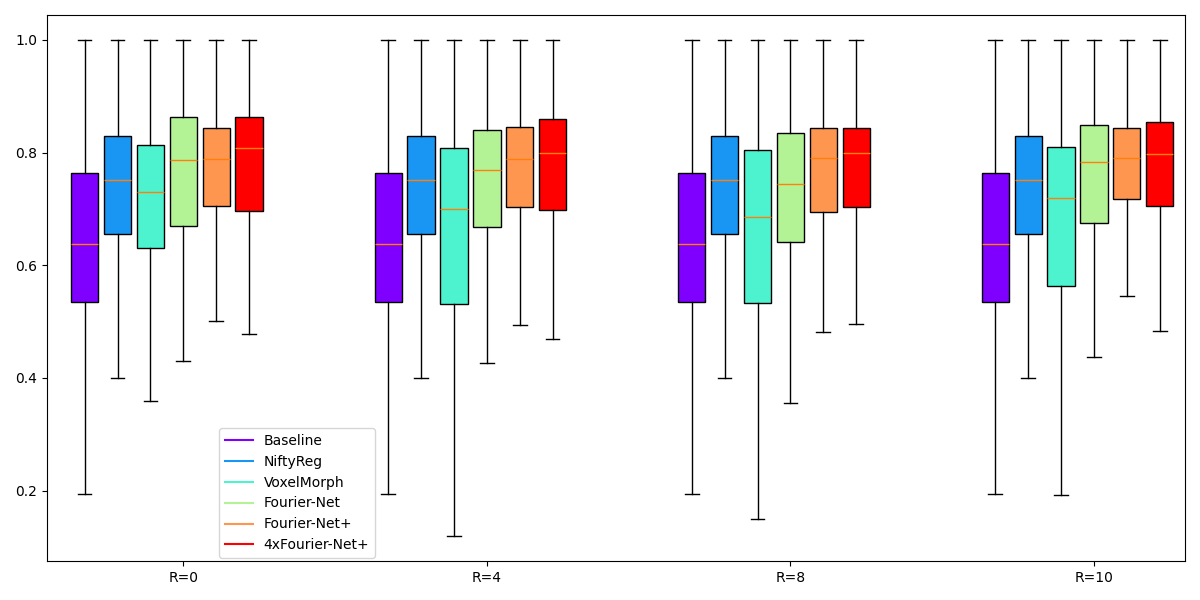
\includegraphics[width=\textwidth]{Boxplot_DiceScores_LV-Cavity.png}
    		\caption{Boxplot of the Dice scores for the left ventricle cavity.} %on the fully sampled \emph{ACDC} test data
    		\label{fig:Boxplot_DiceScores_LV-Cavity}
	\end{subfigure}
	\\
	\begin{subfigure}{0.8\textwidth}
    		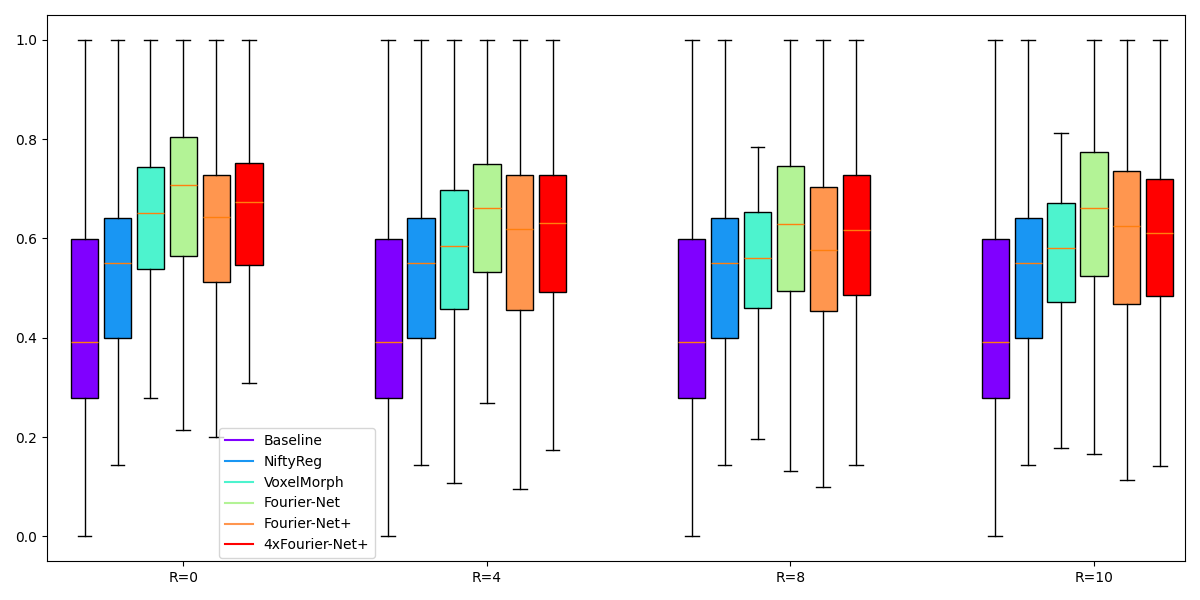
\includegraphics[width=\textwidth]{Boxplot_DiceScores_Myocardium.png}
    		\caption{Boxplot of the Dice scores for the myocardium.} %on the Acc4 \emph{ACDC} test data
    		\label{fig:Boxplot_DiceScores_Myocardium}
	\end{subfigure}
	\\
	\begin{subfigure}{0.8\textwidth}
    		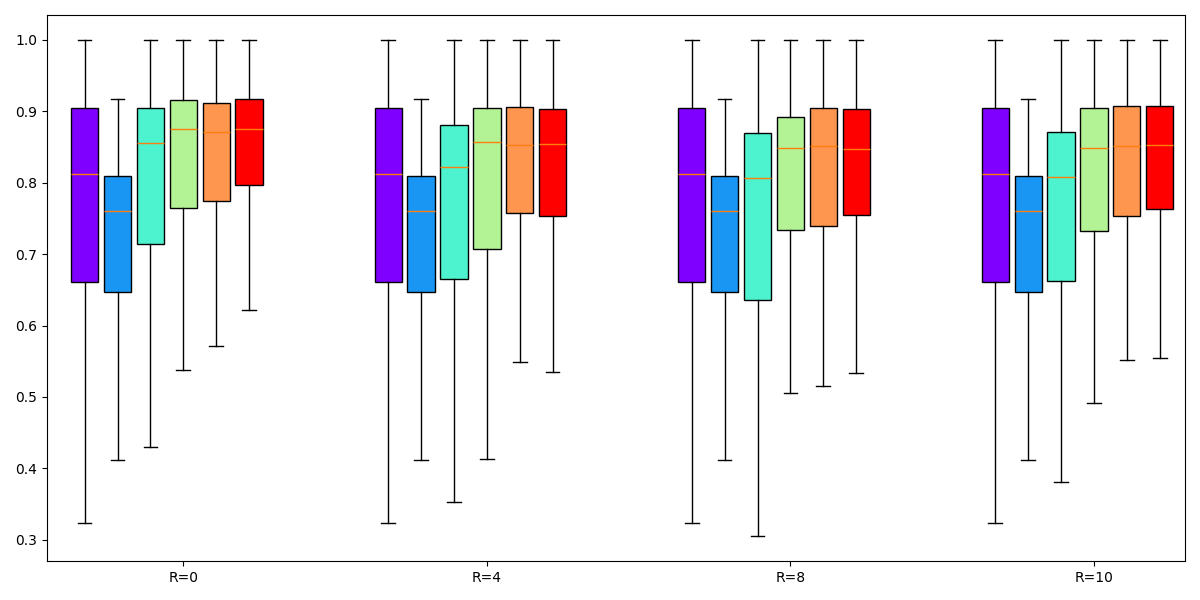
\includegraphics[width=\textwidth]{Boxplot_DiceScores_RV-Cavity.png}
    		\caption{Boxplot of the Dice scores for right ventricle cavity.} %on the Acc8 \emph{ACDC} test data
    		\label{fig:Boxplot_DiceScores_RV-Cavity}
	\end{subfigure}
	\caption{Boxplots of Dice scores (split by label excluding the background) for all models on fully sampled ($R=0$) and subsampled ($R=4$, $R=8$, $R=10$) \emph{ACDC} test data.}
	\label{fig:Boxplots_DiceScores}
\end{figure}

%\begin{figure}[h] %tpb
%	\centering
%	\graphicspath{{images/}{\main/images/}}
%	\begin{subfigure}{\textwidth}
%    		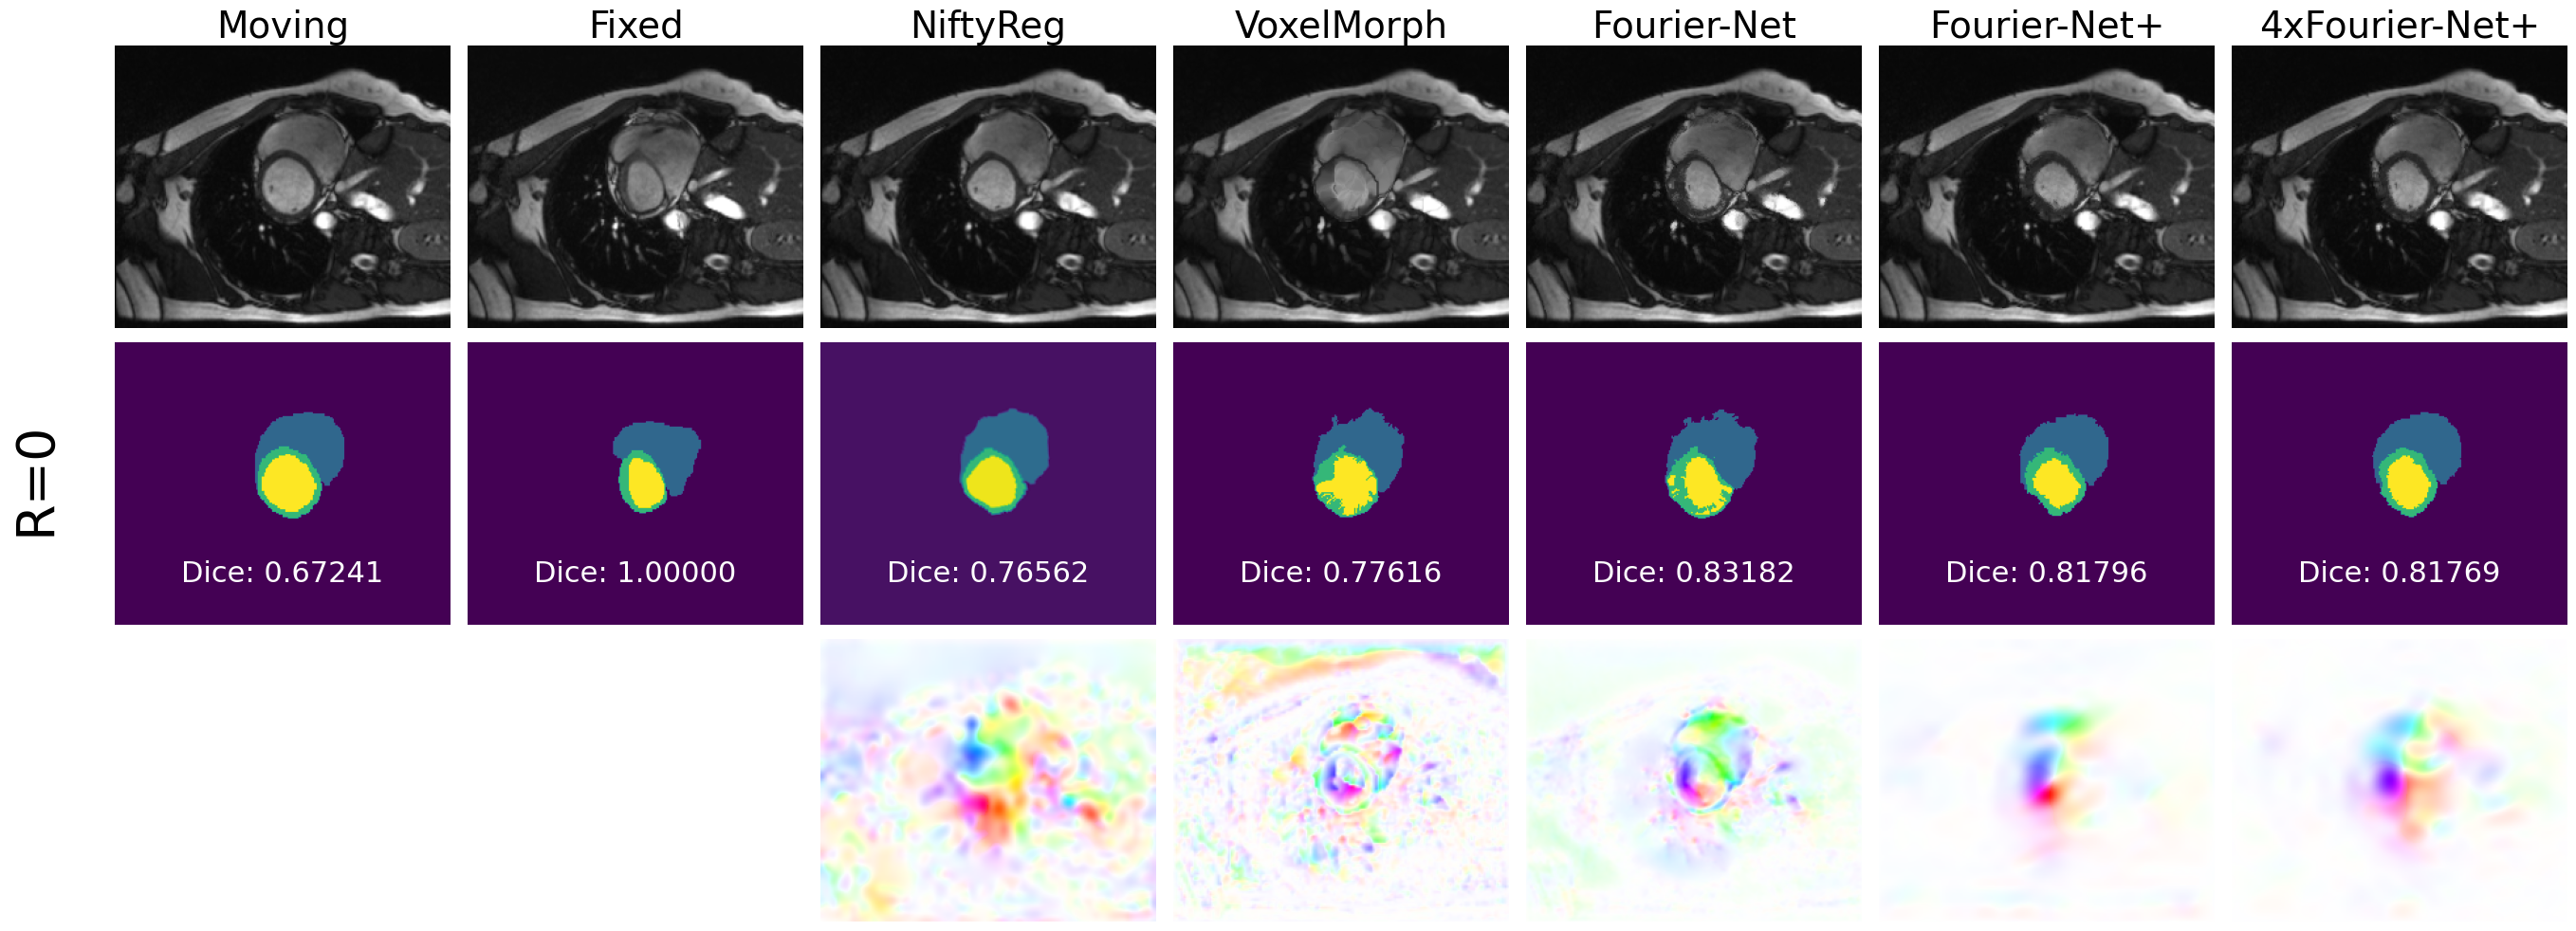
\includegraphics[width=\textwidth]{TestExamples_Mode0.png}
%    		\caption{Example images and segmentations for fully sampled ($R=0$) data.}
%    		\label{fig:TestExamples_Mode0}
%	\end{subfigure}
%	\\
%	\begin{subfigure}{\textwidth}
%    		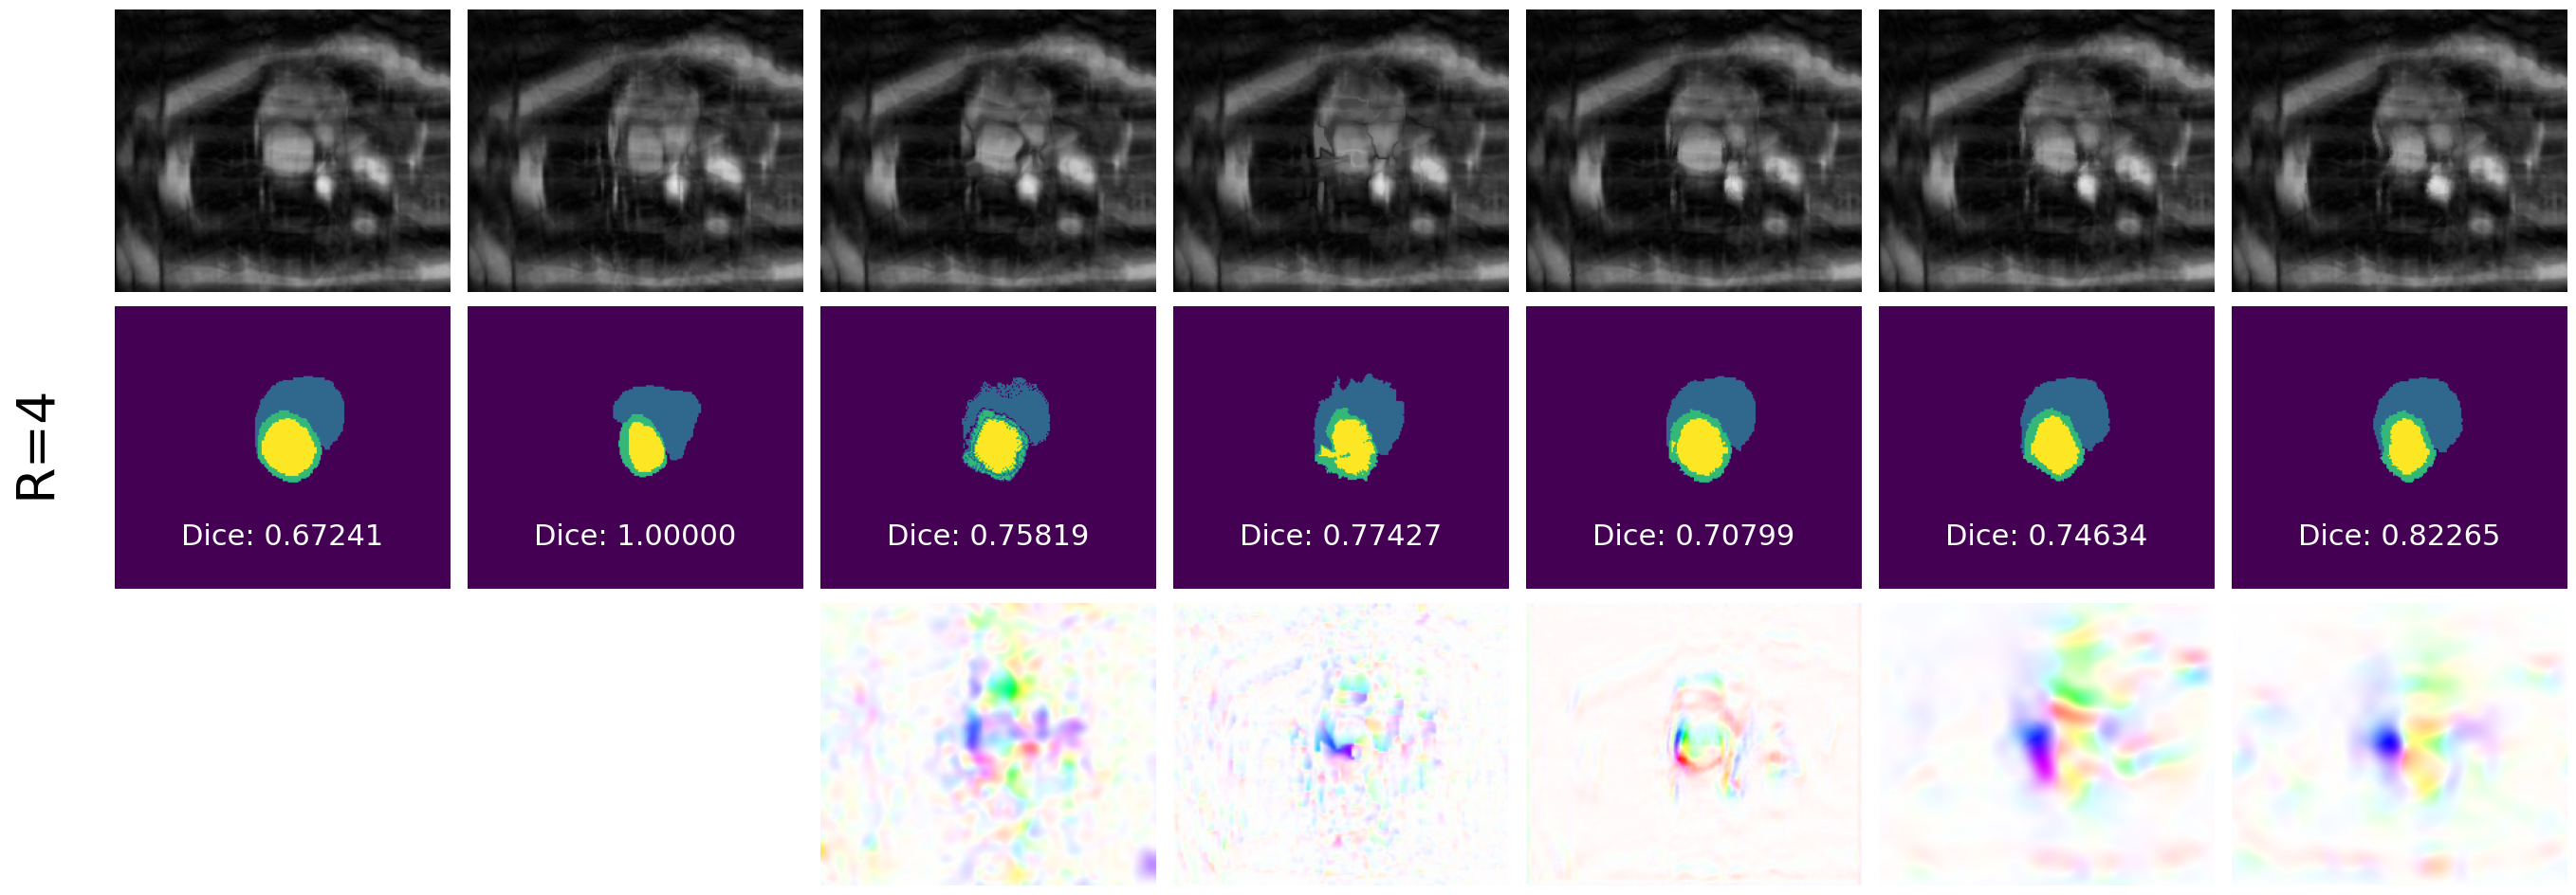
\includegraphics[width=\textwidth]{TestExamples_Mode1.png}
%    		\caption{Example images and segmentations for Acc4 ($R=4$) data.}
%    		\label{fig:TestExamples_Mode1}
%	\end{subfigure}
%	\\
%	\begin{subfigure}{\textwidth}
%    		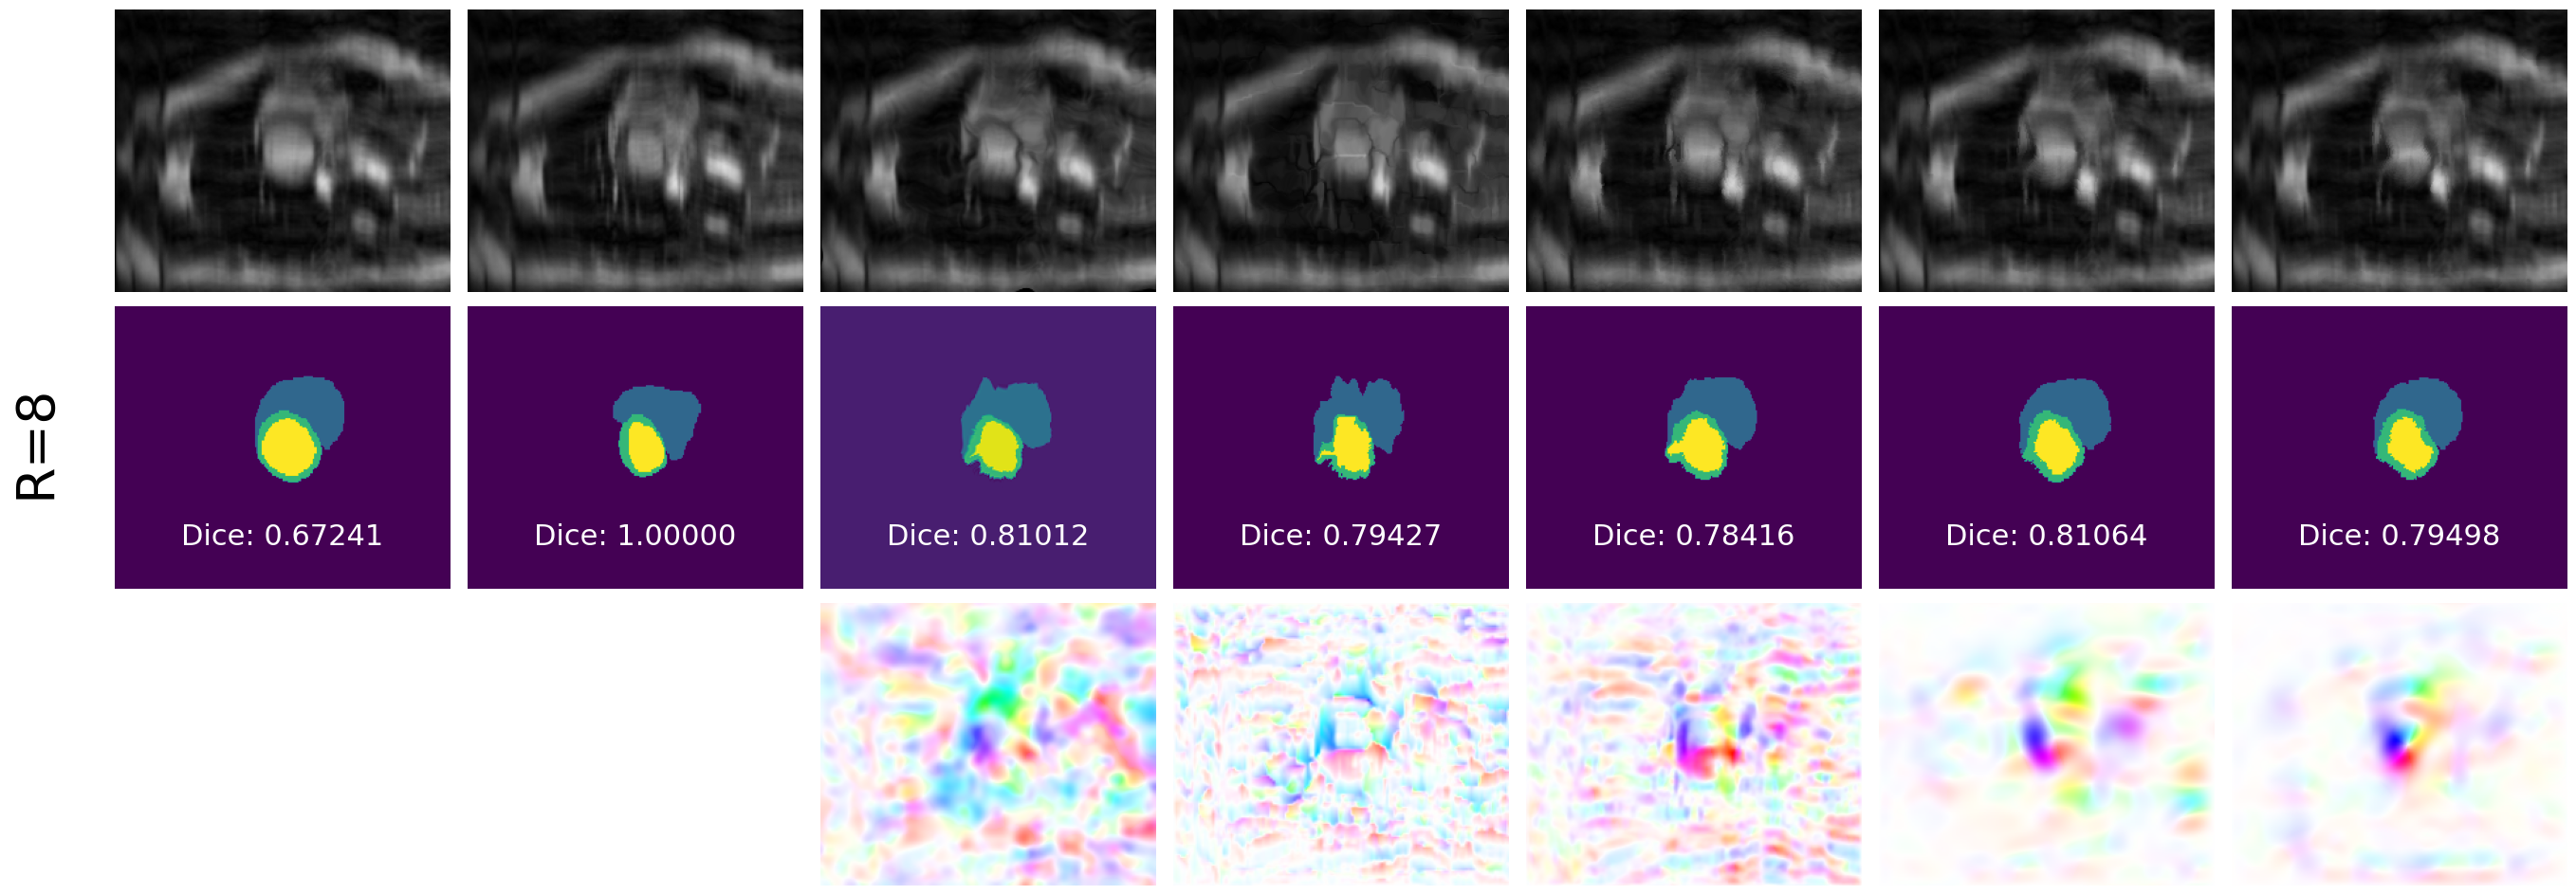
\includegraphics[width=\textwidth]{TestExamples_Mode2.png}
%    		\caption{Example images and segmentations for Acc8 ($R=8$) data.}
%    		\label{fig:TestExamples_Mode2}
%	\end{subfigure}
%	\\
%	\begin{subfigure}{\textwidth}
%    		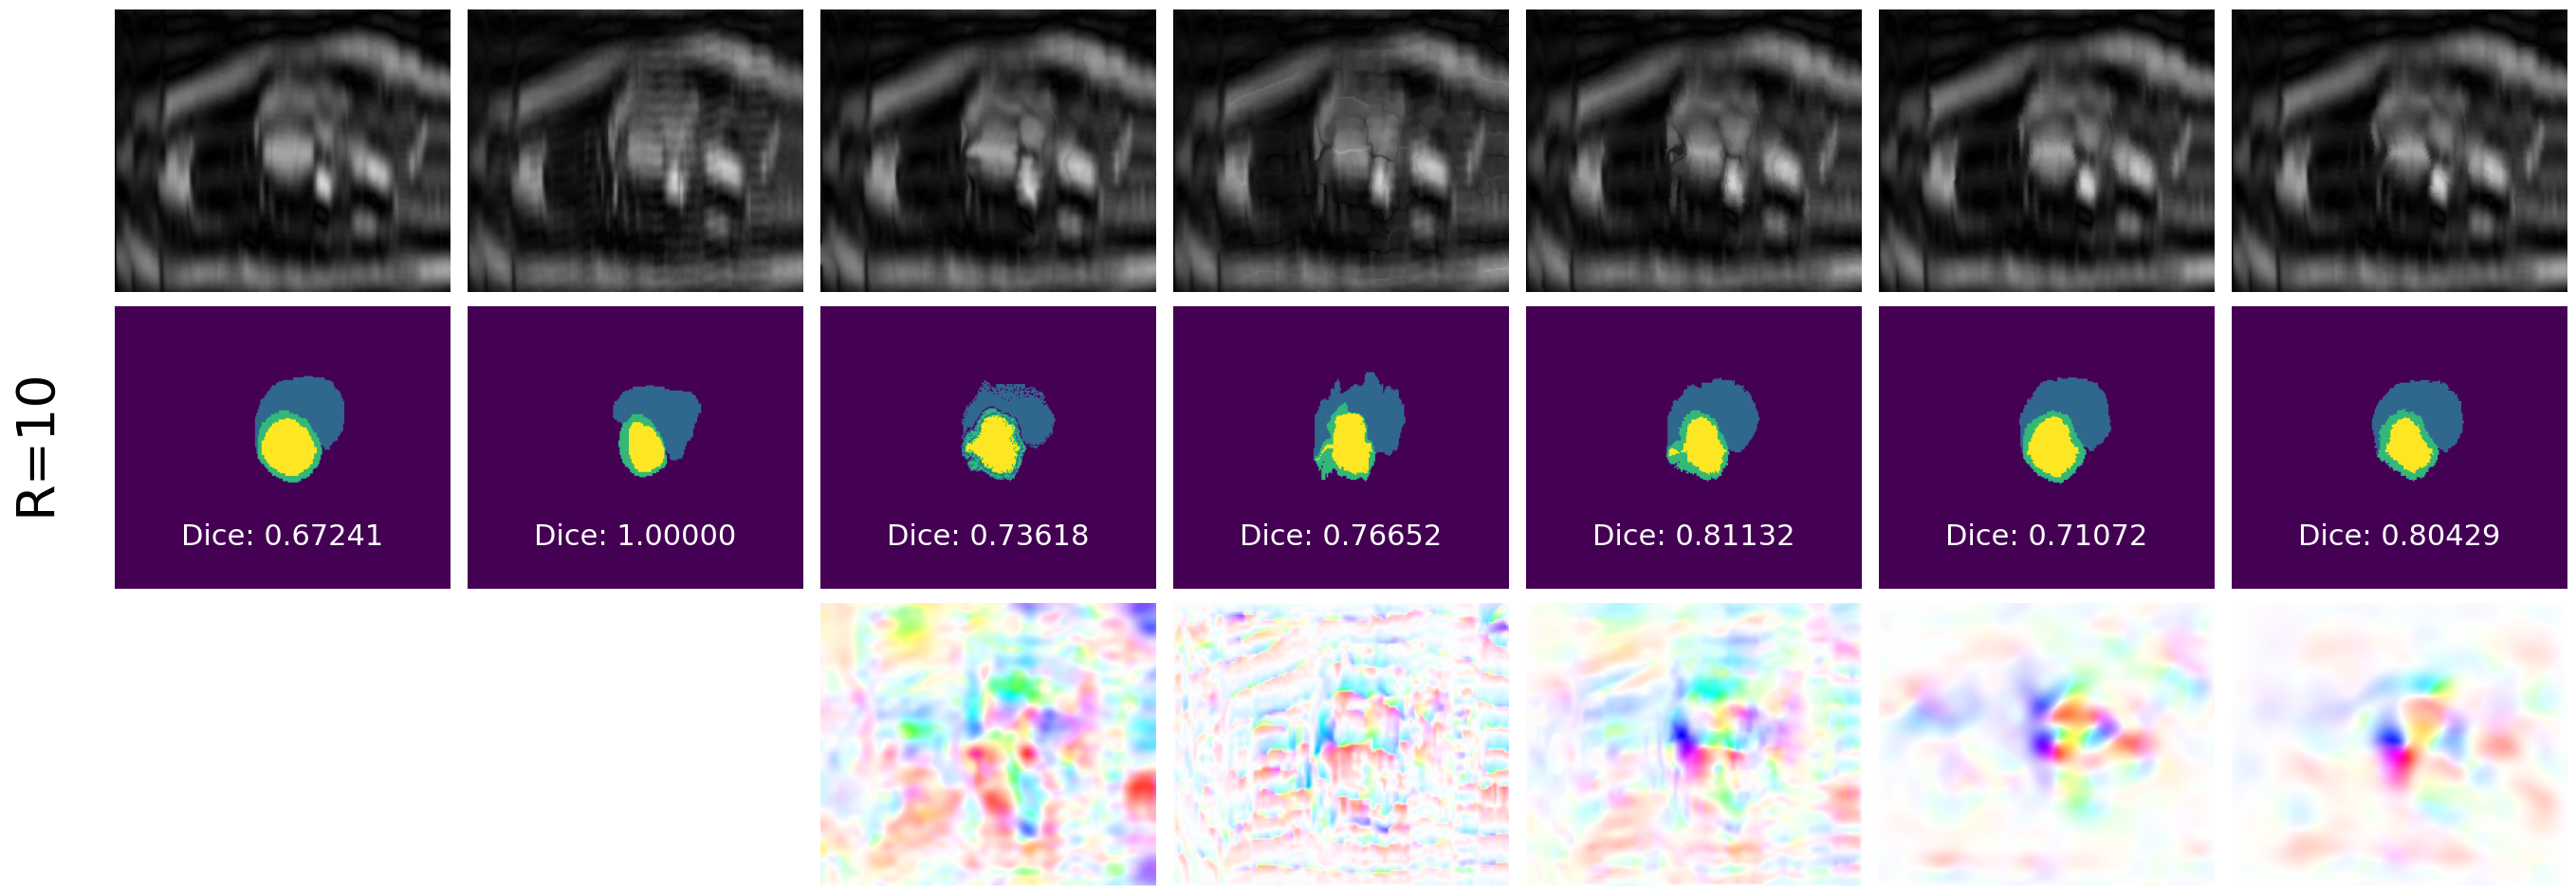
\includegraphics[width=\textwidth]{TestExamples_Mode3.png}
%    		\caption{Example images and segmentations for Acc10 ($R=10$) data.}
%    		\label{fig:TestExamples_Mode3}
%	\end{subfigure}
%	\caption{Examples of warped images and segmentations for \emph{NiftiReg}, \emph{VoxelMorph}, \emph{Fourier-Net}, \emph{Fourier-Net+} and \emph{4xFourier-Net+} together with the original image pair from the \emph{ACDC} test data.}
%	\label{fig:TestExamples}
%\end{figure}


\subsubsection{Qualitative Results}
In order to explain the differences observed between the methods previously, a visual examination can be used. There, one can look at the warped images and segmentations as well as the generated displacement fields visualized in Figure~\ref{fig:TestExamples}. For all acceleration factors, an example moving and fixed image can be compared to the warped images by the different methods. For further analysis, the corresponding segmentations (with corresponding Dice scores) and displacement fields generated by the methods are given.\\
For $R=0$, \emph{Fourier-Net+} and \emph{4xFourier-Net+} have very localized displacements, centered on the cardiac region, leading to a very smooth warped segmentation compared to \emph{Fourier-Net} and \emph{VoxelMorph} where the cardiac labels mix in some regions. Despite this, \emph{Fourier-Net} still achieves the highest Dice score with an $16\%$ increase compared to the baseline. While \emph{NiftyReg} does produce a very smooth warped segmentation the actual displacements are very small and not localized on the cardiac region leading to the lowest Dice score of all methods.\\
For $R=4$, the image artifacts due to the subsampling are very apparent. The segmentations for the moving and fixed image obviously remain the same.
% despite the subsampling.
\emph{Fourier-Net+} and \emph{4xFourier-Net+} again have very smooth segmentations, however the displacements reflect the difficulties of adapting to subsampled data in becoming slightly less local. Surprisingly, \emph{NiftyReg} actually has a more localized displacement compared to the fully sampled data, however the segmentation looks less smooth and the Dice score is slightly lower. Somewhat similar, \emph{VoxelMorph} also has a more localized displacement leading to a smoother segmentation and a higher Dice score. The results of \emph{Fourier-Net} look overall very similar to the fully sampled case, perhaps with a bit more localized displacement leading to a smoother segmentation, although this does not lead to a better Dice Score.\\
For $R=8$, the displacements for all methods become more global due to the strong presence of image artifacts, however the Dice scores are higher than before for all methods. \emph{NiftyReg} even outperforms \emph{VoxelMorph} for the first time. This trend does not continue for $R=10$ however, were \emph{NiftyReg} is again far behind all other methods in terms of Dice with a very much more global displacement. \emph{VoxelMorph} seems to compensate more for the rippling artifacts present in the fixed image than for the change in the cardiac region as seen in the displacement. \emph{Fourier-Net}, \emph{Fourier-Net+} and \emph{4xFourier-Net+} do not share this behavior although their displacements also become more global and less focused on the cardiac region. The latter network has the highest Dice score for the first time managing an increase in Dice of about $16\%$ compared to the baseline for this specific case despite the heavy subsampling showing the robustness of the network.

\begin{figure}[H]
	\centering
	\graphicspath{{images/}{\main/images/}}
	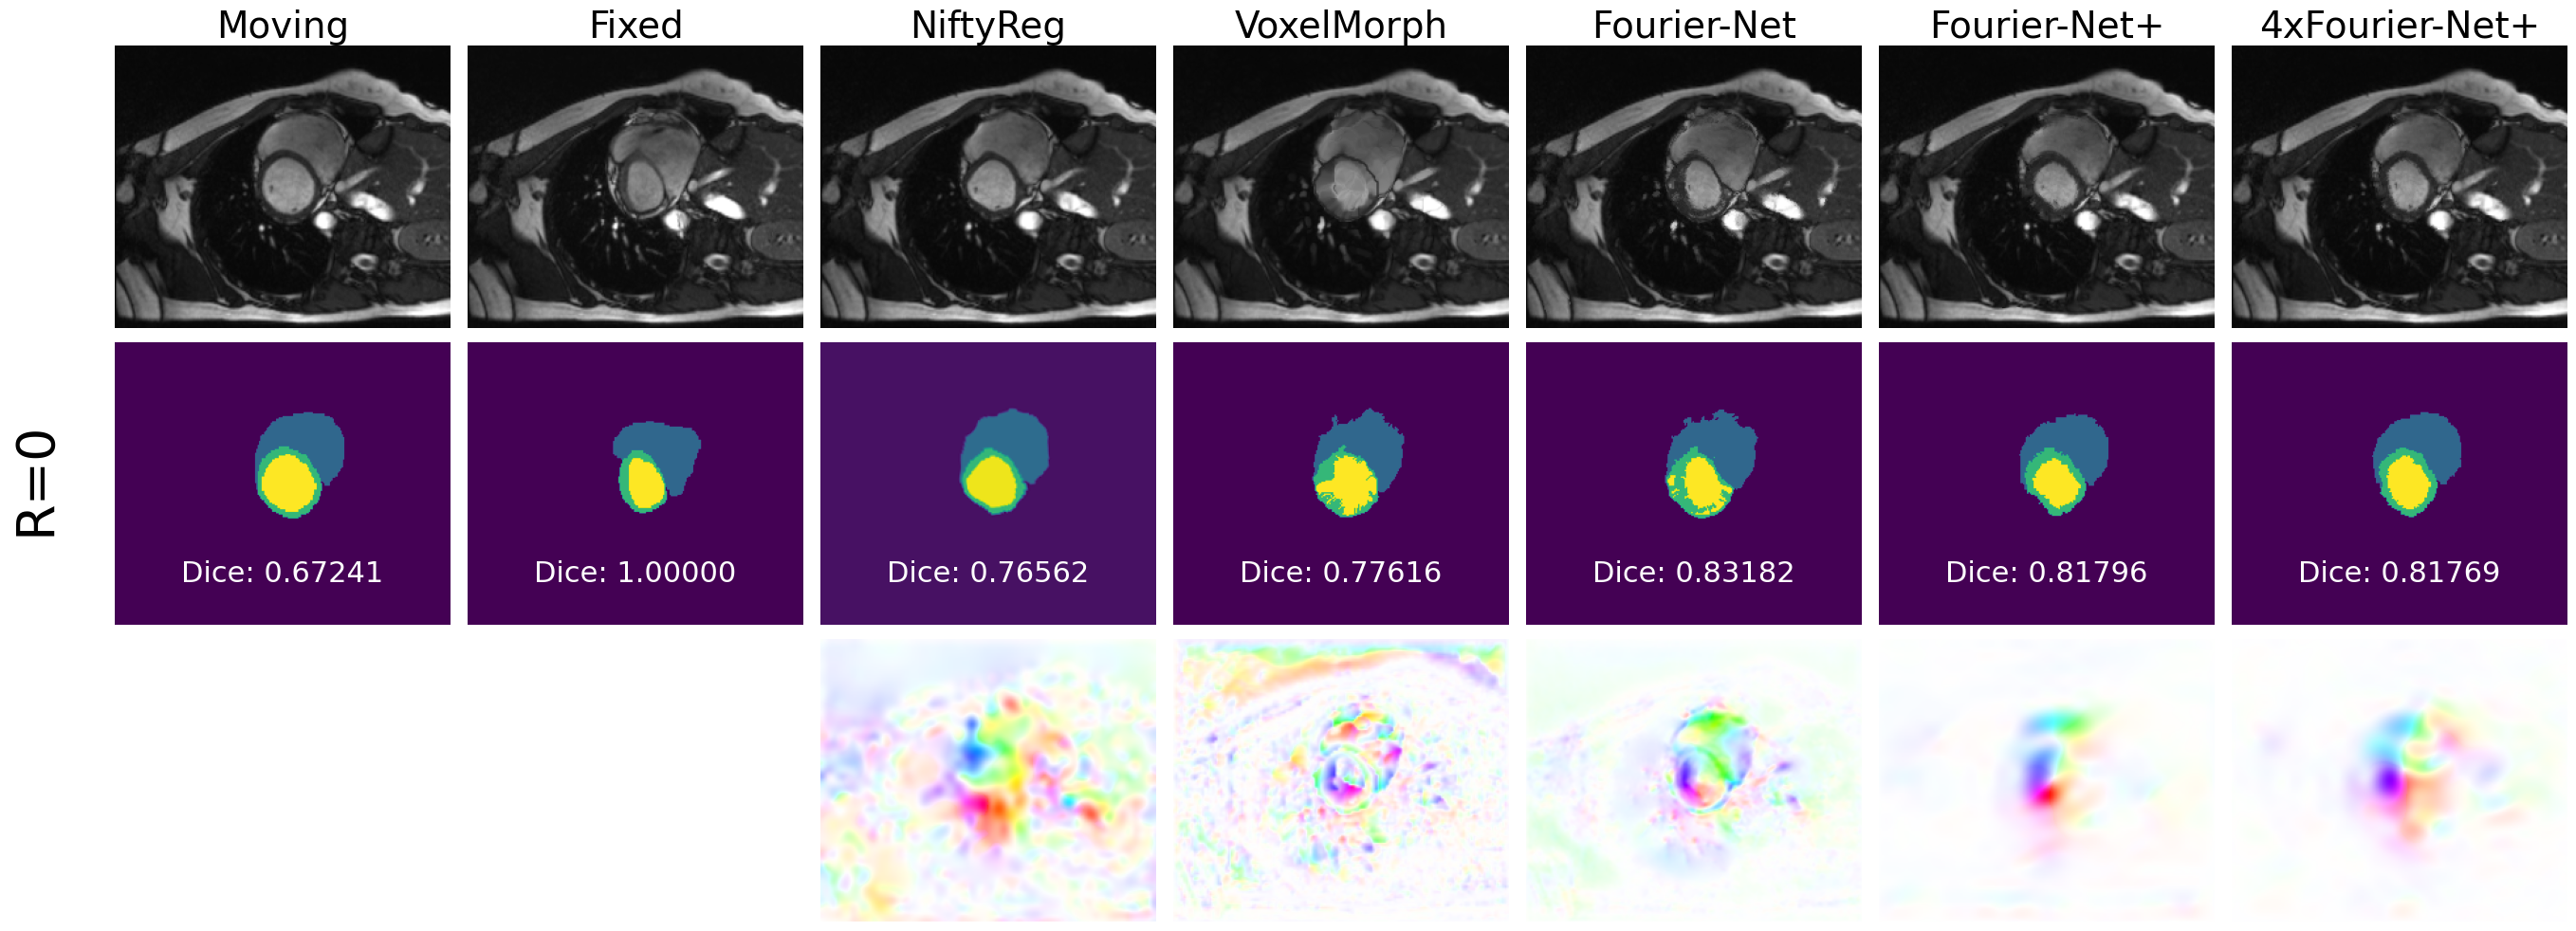
\includegraphics[width=\textwidth]{TestExamples_Mode0.png}
    	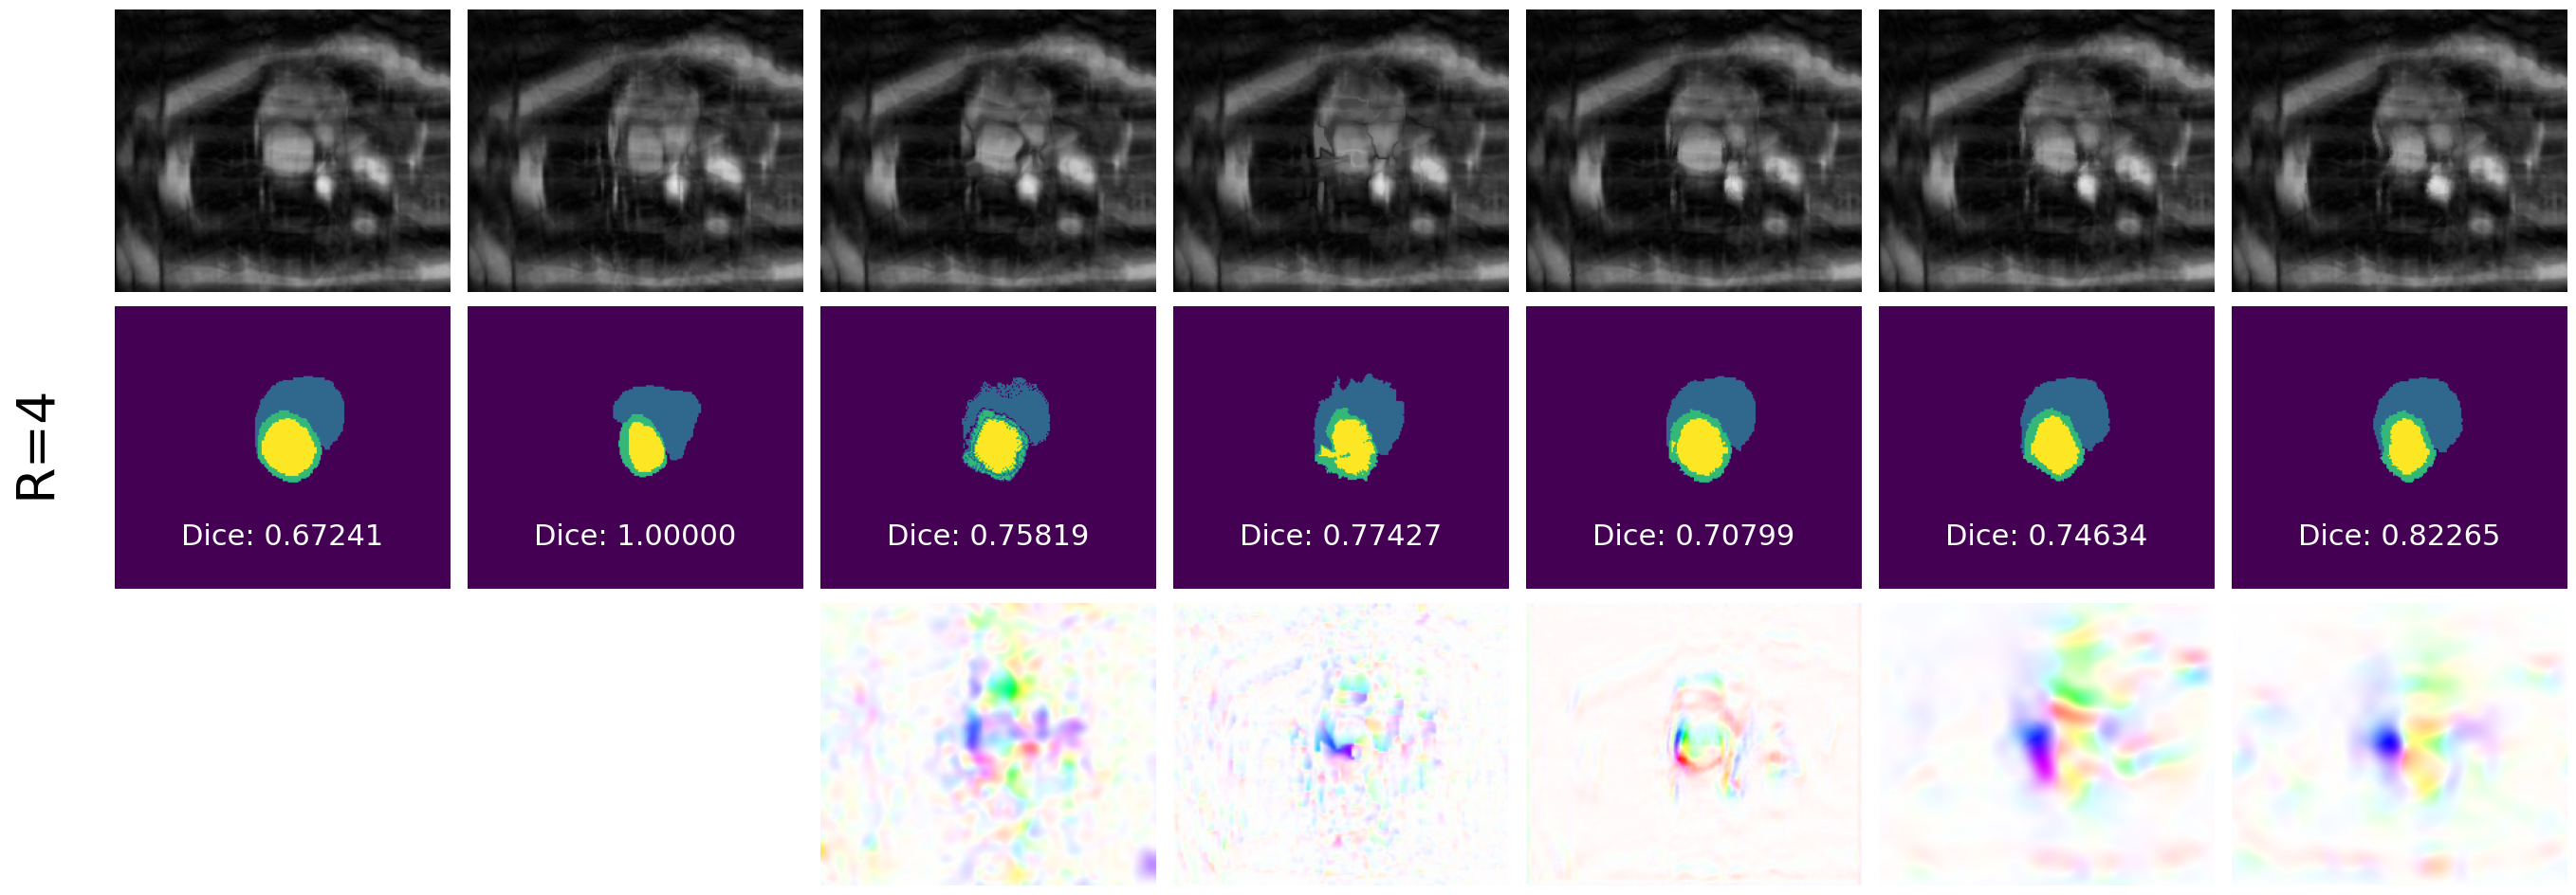
\includegraphics[width=\textwidth]{TestExamples_Mode1.png}
    	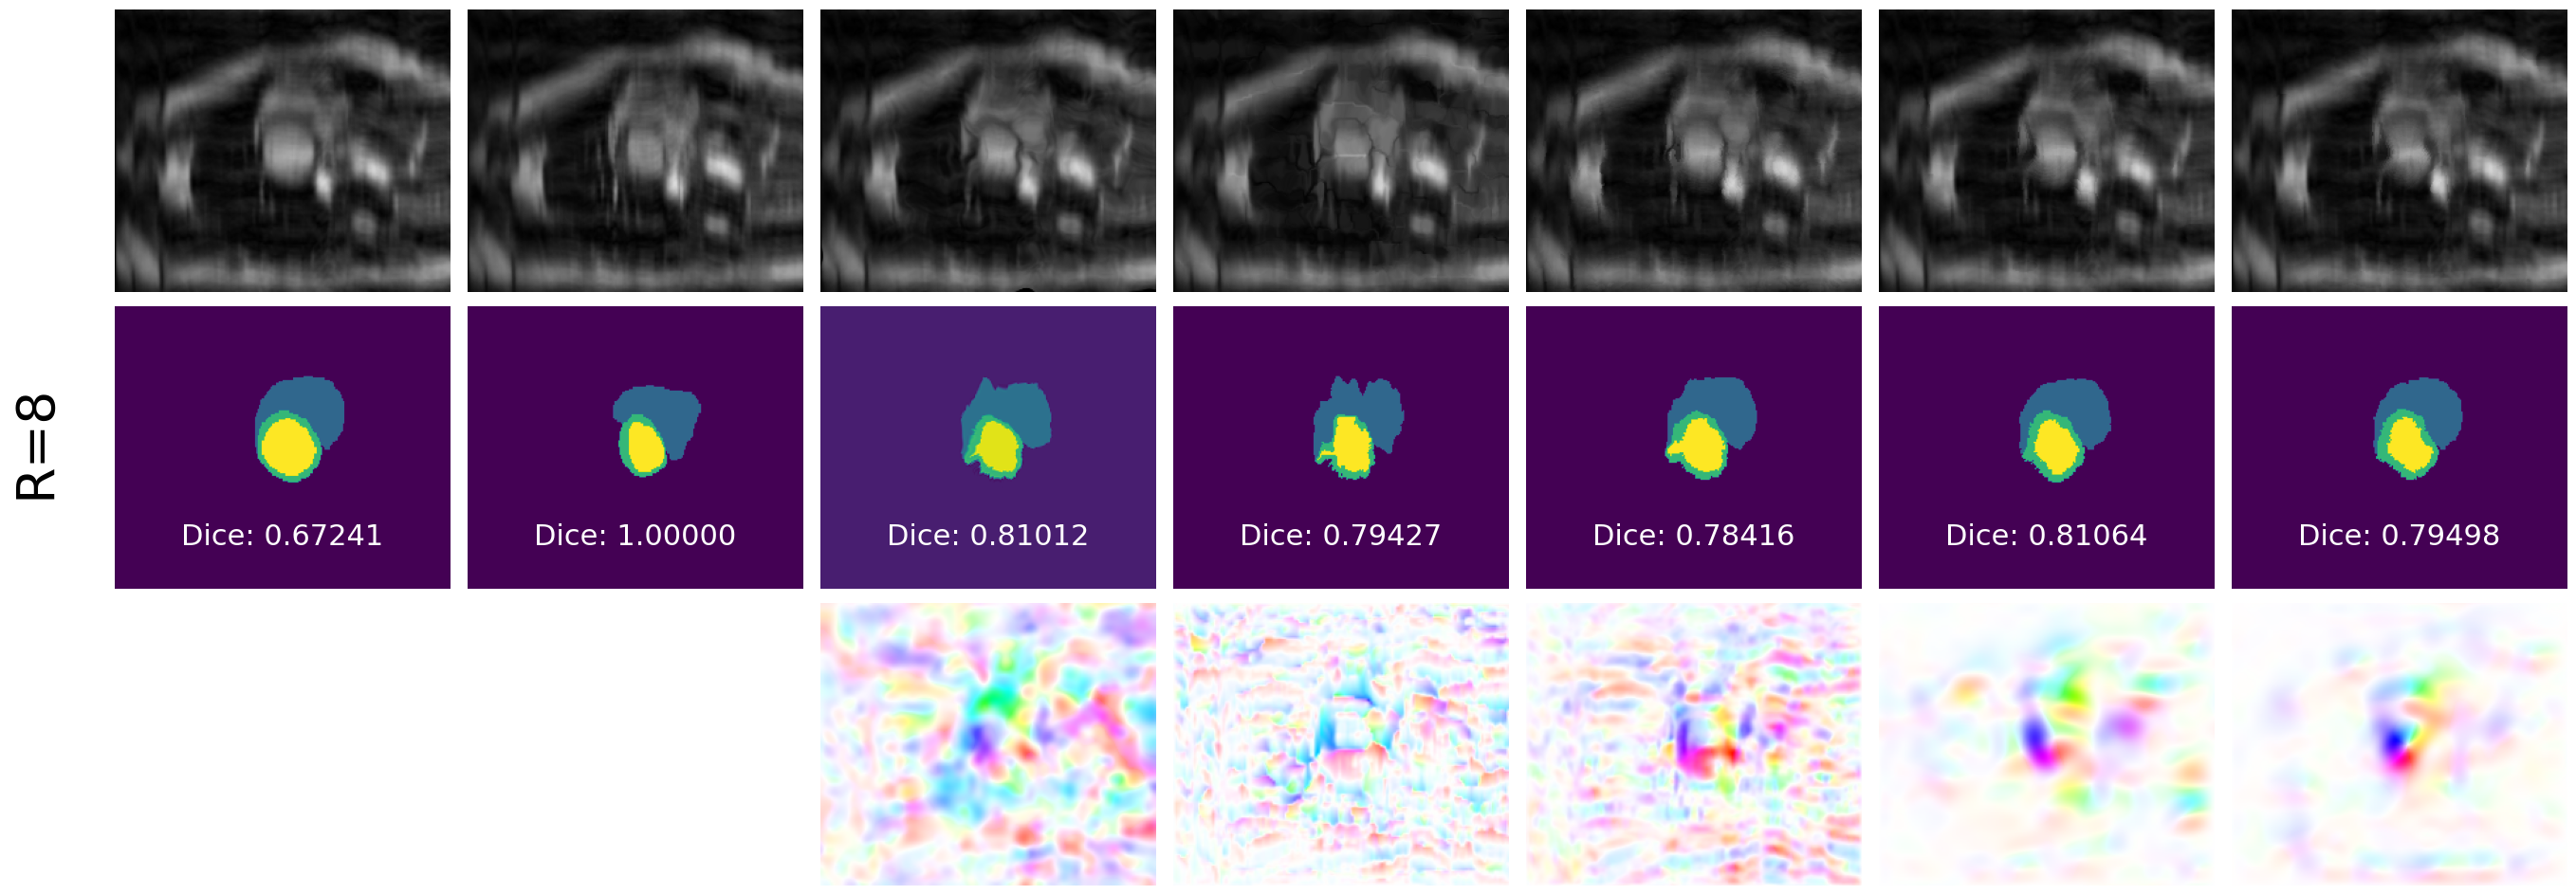
\includegraphics[width=\textwidth]{TestExamples_Mode2.png}
    	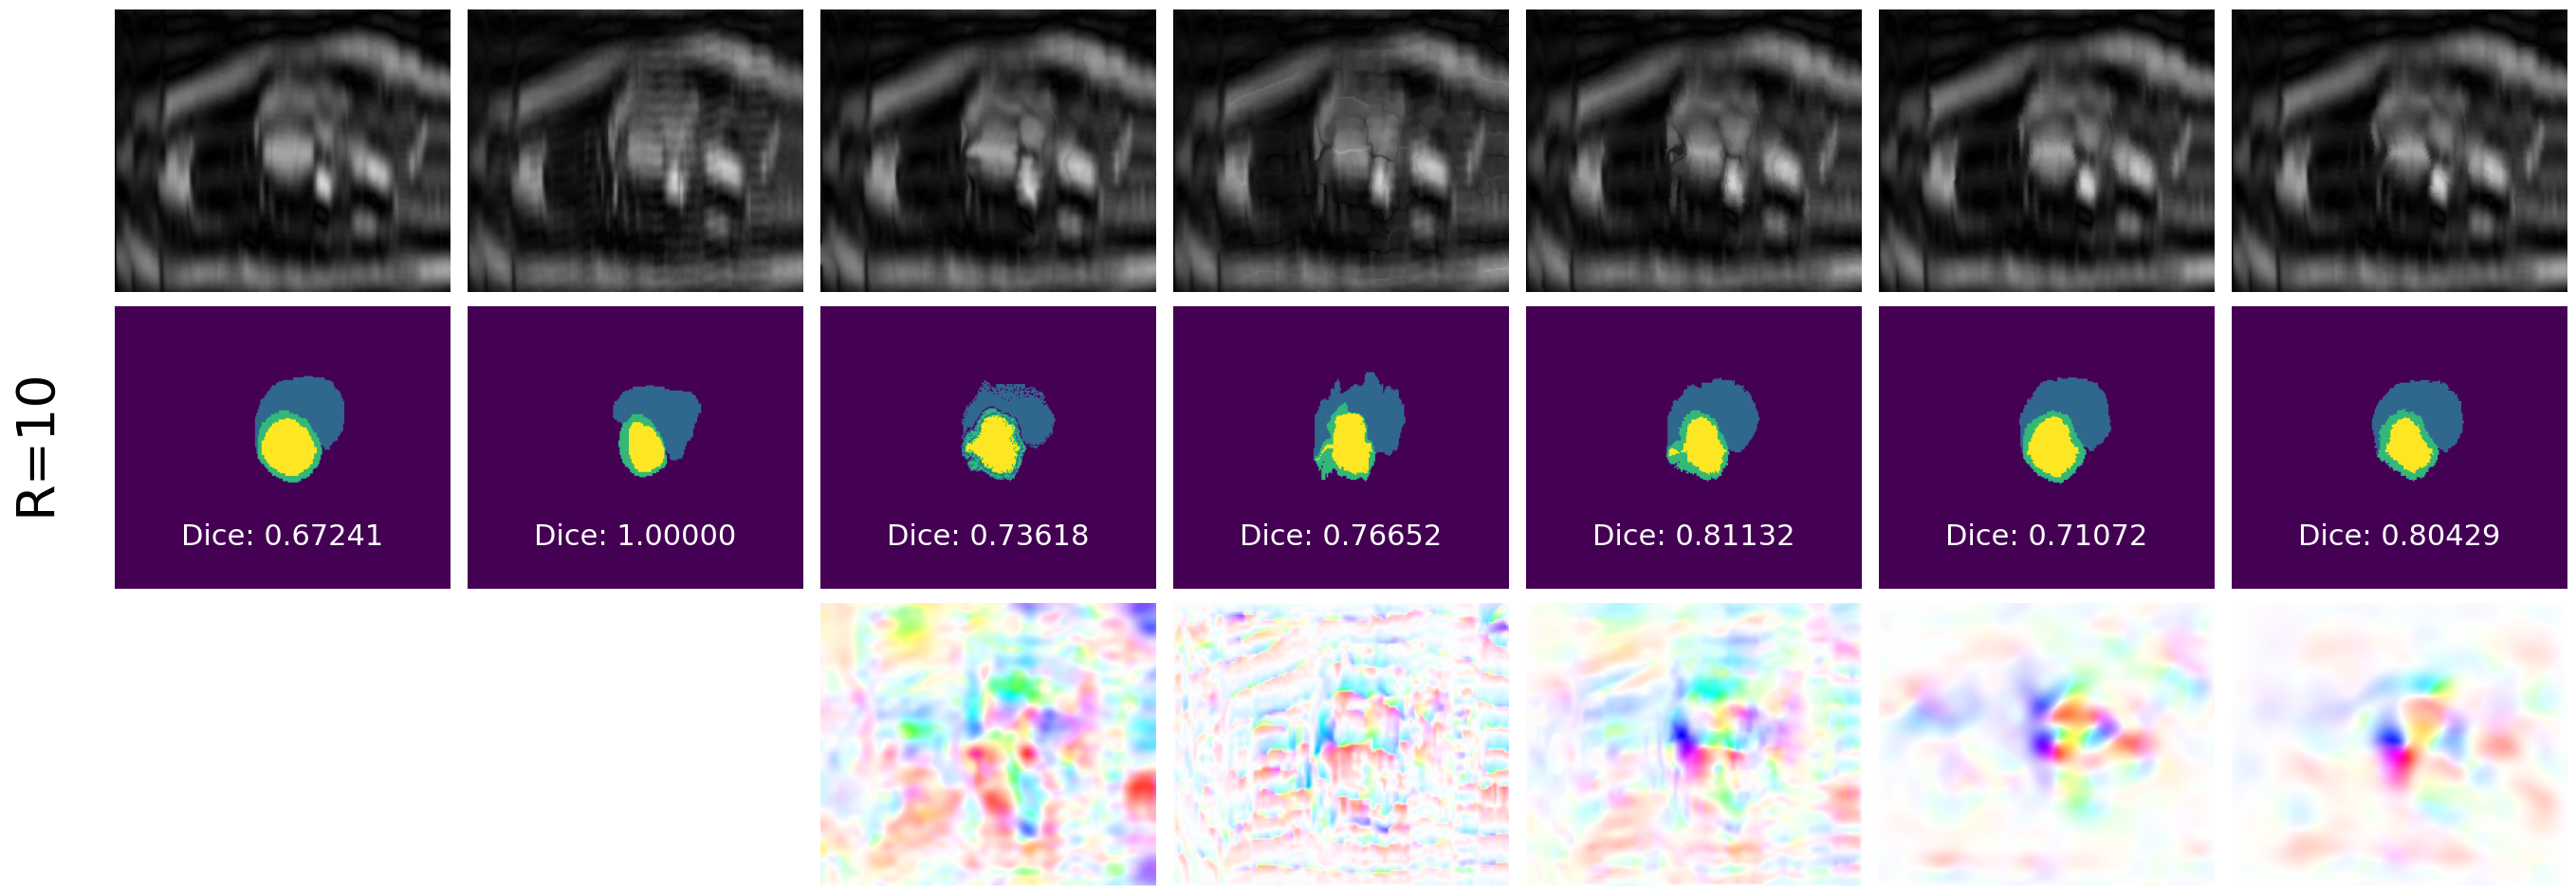
\includegraphics[width=\textwidth]{TestExamples_Mode3.png}	
	\caption{Examples of warped images, segmentations and flow fields for \emph{NiftiReg}, \emph{VoxelMorph}, \emph{Fourier-Net}, \emph{Fourier-Net+} and \emph{4xFourier-Net+} together with the original image pair from the fully sampled ($R=0$) and subsampled ($R=4$, $R=8$, $R=10$) \emph{ACDC} test data.}
	\label{fig:TestExamples}
\end{figure}


\section{Integration into a Motion-Compensated Reconstruction Pipeline} \label{Sec:ResultsIntegrationMotion-CompensatedReconstructionPipeline}
After assessing the registration performance of \emph{Fourier-Net}, \emph{Fourier-Net+} and \emph{4xFourier-Net+}, a final down-stream task to gauge the applicability of these networks was conducted in the form of an motion-compensated reconstruction pipeline where the networks are used to correct the moment between frames.

\subsection{Domain Translation} \label{SubSec:ResultsDomainTranslation}
First, the domain gap between the \emph{ACDC} and \emph{CMRxRecon} dataset was of interest. To estimate the generalizability of our previous results on the new cardiac dataset 
\emph{Fourier-Net}, \emph{Fourier-Net+} and \emph{4xFourier-Net+} were trained again on the accelerated \emph{CMRxRecon} data. They were then compared to the \emph{Fourier-Net}, \emph{Fourier-Net+} and \emph{4xFourier-Net+} version which were previously trained for 6 epochs on \emph{ACDC}. All other network parameters were held constant for comparability. The results can be seen in Table~\ref{tab:DomainTranslation_ACDC_CMRxRecon}.\\
For \emph{Fourier-Net+} and \emph{4xFourier-Net+}, the metrics barely change between the versions trained on \emph{ACDC} and \emph{CMRxRecon}. The MSE is negligible at $0.01 \cdot 10^{-3}$, the SSIM is at a high mean value of $97.88 \%$ with the Jacobian detminants showing no folding. The only difference are slight changes in the standard deviation of the SSIM and the inference time of each method. \emph{Fourier-Net+} is faster on \emph{ACDC} while \emph{4xFourier-Net+} is faster on \emph{CMRxRecon}. Overall, only \emph{Fourier-Net} shows a difference in similarity metrics between datasets with an SSIM of $97.99 \%$, MSE of $0.01 \cdot 10^{-3}$ and no folding on \emph{CMRxRecon} similar to \emph{Fourier-Net+} and \emph{4xFourier-Net+}, while the SSIM improves to $98.21 \%$ on \emph{ACDC} with no change in MSE and a slight increase with $0.03 \%$ non-positive Jacobian determinants. \emph{Fourier-Net}, similar to \emph{4xFourier-Net+}, also is slightly faster on \emph{CMRxRecon}.

\begin{table}[H] %tpb
	%\scriptsize
	\centering
	\caption{Results for \emph{Fourier-Net}, \emph{Fourier-Net+} and \emph{4xFourier-Net+} trained on the $R=4$ \emph{ACDC} and \emph{CMRxRecon} data and tested on the $R=4$ \emph{CMRxRecon} test data.}
	\label{tab:DomainTranslation_ACDC_CMRxRecon}
	\begin{tabularx}{\textwidth}{Y Y Y Y} 
		\toprule
		\multirow{2}{*}{Metrics} & \multicolumn{3}{c}{Trained on \emph{ACDC}} \\
		\cmidrule(lr){2-4} 
		 & Fourier-Net & Fourier-Net+ & 4xFourier-Net+\\	
		\midrule
		$\%$ SSIM $\uparrow$ & \textbf{98.21} $\pm$ \textbf{1.07} & $97.88 \pm 1.04$ & $97.88 \pm 1.04$\\
		MSE (m) $\downarrow$ & $0.01 \pm 0.01$ & $0.01 \pm 0.01$ & $0.01 \pm 0.01$ \\
		$\% \, |J_{\phi}|\leq0 \downarrow$ & $0.03 \pm 0.09$ & \textbf{0.00} $\pm$ \textbf{0.00} & \textbf{0.00} $\pm$ \textbf{0.00} \\
		Time [ms] $\downarrow$ 	  & 3.81 & \textbf{3.72} & 18.52  \\
		\midrule
		\multirow{2}{*}{Metrics} & \multicolumn{3}{c}{Trained on \emph{CMRxRecon}} \\
		\cmidrule(lr){2-4} 
		 & Fourier-Net & Fourier-Net+ & 4xFourier-Net+\\		
		\midrule
		$\%$ SSIM $\uparrow$ & \textbf{97.99} $\pm$ \textbf{1.04} & $97.88 \pm 1.06$ & $97.88 \pm 1.07$\\
		MSE (m) $\downarrow$ & $0.01 \pm 0.01$ & $0.01 \pm 0.01$ & $0.01 \pm 0.01$ \\
		$\% \, |J_{\phi}|\leq0 \downarrow$ & $0.00 \pm 0.01$ & $0.00 \pm 0.00$ & $0.00 \pm 0.00$ \\
		Time [ms] $\downarrow$ 	  & \textbf{2.86} & 4.32 & 12.61  \\
		\bottomrule
	\end{tabularx}	
\end{table}


\subsection{Reconstruction Pipeline} \label{SubSec:ResultsReconstructionPipeline}
After ensuring that the previous results were translatable to the new data, the reconstruction pipeline had to be evaluated. As the \emph{CMRxRecon} dataset does not include segmentations for Dice calculation, image similarity metrics need to be utilized. For this, SSIM and MSE were used again, however, the PSNR (see section~\ref{SubSec:NetworkTrainingAndTesting}) and HaarPSI~\cite{HaarPSI} were also added. 

\subsubsection{K-Space Line Swapping}
After ensuring that the reconstruction pipeline worked, the input images were further corrupted as the cardiac motion present was not deemed severe enough. To simulate motion or mis-triggering a similar strategy to~\cite{Oksuz2020} was used, swapping $z=\{16,32\}$ k-space lines between the frames. Results for the motion-compensated reconstruction using \emph{VoxelMorph}, \emph{Fourier-Net}, \emph{Fourier-Net+} and \emph{4xFourier-Net+} are shown in Table~\ref{tab:ComparisonReconstructionCMRxReconLineSwapping} with blue marking the best results per metric (not present if all methods have the same performance) and red marking worse results than the baseline.\\
For $z=16$, performance decreases with higher acceleration. For $R=4$, \emph{Fourier-Net} has the highest HaarPSI and SSIM values, while \emph{VoxelMorph} has the highest PSNR. \emph{Fourier-Net+} on the other hand, has the lowest values for these metrics. All methods as well as the baseline have the same mean MSE value. Only for the third decimal point in the standard deviation a small difference between the different methods is visible (note that the MSE values are already multiplied by a factor of 100). %\\
For $R=8$, \emph{Fourier-Net} again has the highest value for the HaarPSI, followed by \emph{Fourier-Net+}, as well as the highest SSIM value, followed by \emph{4xFourier-Net+} which also has the highest PSNR. While the MSE values are again very close, \emph{4xFourier-Net+} has a slightly lower mean value than the other methods.%\\
For $R=10$, \emph{4xFourier-Net+} performs best for all metrics with \emph{Fourier-Net+} having the same mean MSE value. \emph{VoxelMorph} and \emph{Fourier-Net} perform worse than baseline for the HaarPSI with the latter also having lower PSNR and SSIM values than the baseline.\\
For $z=32$ and $R=4$, \emph{Fourier-Net} performs best for all metrics, while \emph{4xFourier-Net+} performs worse than baseline for PSNR, SSIM and MSE. For $R=8$, \emph{Fourier-Net+} has the highest HaarPSI, PSNR and SSIM values followed by \emph{Fourier-Net}. The mean MSE value is again the same for all methods and slightly lower than the baseline. For $R=10$, \emph{Fourier-Net+} again performs best for all metrics. Only \emph{Fourier-Net} has a lower SSIM than the baseline.

\begin{table}[H] %tpb
	%\footnotesize
	\small
	\centering
	\caption{Reconstruction results \emph{VoxelMorph}, \emph{Fourier-Net}, \emph{Fourier-Net+} and \emph{4xFourier-Net+} on the \emph{CMRxRecon} test data for $R=4$, $R=8$ and $R=10$ as well as an baseline without motino-correction. The best results for each metric and subsampling are highlighted in blue, while values worse than the unaligned baseline are marked with red.}
	\label{tab:ComparisonReconstructionCMRxReconLineSwapping}
	\begin{tabularx}{\textwidth}{c Y Y Y Y Y} 
		\toprule
		 & \multirow{2}{*}{Methods} & \multicolumn{4}{c}{Motion-correction for $z=16$ swapped k-space lines} \\
		\cmidrule(lr){3-6} 
		 & & $\%$ HaarPSI $\uparrow$ & PSNR [dB] $\uparrow$ & $\%$ SSIM $\uparrow$ & MSE (m) $\downarrow$\\
		
		% 4x Accelerated (R=4) 				 		
		\midrule
		\multirow{5}{*}{\rotatebox{90}{$R=4$}} & Baseline & $56.884 \pm 8.129$ & $28.703 \pm 2.388$ & $78.079 \pm 5.887$ & $0.160 \pm 0.125$ \\  
		 & VoxelMorph & $56.909 \pm 8.118$ & \textcolor{blue}{$28.709 \pm 2.404$} & $78.090 \pm 5.903$ & $0.160 \pm 0.126$ \\  
		 & Fourier-Net & \textcolor{blue}{$56.918 \pm 8.160$} & $28.706 \pm 2.401$ & \textcolor{blue}{$78.123 \pm 5.893$} & $0.160 \pm 0.126$ \\  
		 & Fourier-Net+ & \textcolor{red}{$56.854 \pm 8.158$} & \textcolor{red}{$28.699 \pm 2.399$} & \textcolor{red}{$78.071 \pm 5.951$} & $0.160 \pm 0.126$ \\   
		 & \mbox{4xFourier-Net+} & $56.903 \pm 8.109$ & $28.702 \pm 2.380$ & $78.085 \pm 5.877$ & $0.160 \pm 0.125$ \\  
		
		% 8x Accelerated (R=8) 
		\midrule
		\multirow{5}{*}{\rotatebox{90}{$R=8$}} & Baseline & $53.318 \pm 7.641$ & $28.104 \pm 2.383$ & $77.311 \pm 5.934$ & $0.183 \pm 0.139$ \\  
		 & VoxelMorph & $53.342 \pm 7.687$ & $28.110 \pm 2.405$ & $77.341 \pm 5.900$ & $0.183 \pm 0.139$ \\  
		 & Fourier-Net & \textcolor{blue}{$53.394 \pm 7.681$} & $28.128 \pm 2.398$ & \textcolor{blue}{$77.416 \pm 5.927$} & $0.183 \pm 0.138$ \\  
		 & Fourier-Net+ & $53.388 \pm 7.664$ & $28.118 \pm 2.404$ & $77.398 \pm 5.906$ & $0.183 \pm 0.138$ \\   
		 & \mbox{4xFourier-Net+} & $53.376 \pm 7.688$ & \textcolor{blue}{$28.133 \pm 2.398$} & $77.402 \pm 5.936$ & \textcolor{blue}{$0.182 \pm 0.138$} \\ 
		 	 
		% 10x Accelerated (R=10) 		 		
		\midrule		
		\multirow{5}{*}{\rotatebox{90}{$R=10$}} & Baseline & $52.212 \pm 7.388$ & $27.906 \pm 2.364$ & $77.175 \pm 5.886$ & $0.191 \pm 0.141$ \\  
		 & VoxelMorph & \textcolor{red}{$52.211 \pm 7.393$} & $27.907 \pm 2.368$ & $77.194 \pm 5.863$ & $0.191 \pm 0.140$ \\  
		 & Fourier-Net & \textcolor{red}{$52.192 \pm 7.361$} & \textcolor{red}{$27.895 \pm 2.362$} & \textcolor{red}{$77.160 \pm 5.815$} & $0.191 \pm 0.139$ \\  
		 & Fourier-Net+ & $52.240 \pm 7.379$ & $27.924 \pm 2.357$ & $77.244 \pm 5.866$ & \textcolor{blue}{$0.189 \pm 0.139$} \\   
		 & \mbox{4xFourier-Net+} & \textcolor{blue}{$52.272 \pm 7.330$} & \textcolor{blue}{$27.931 \pm 2.349$} & \textcolor{blue}{$77.262 \pm 5.816$} & \textcolor{blue}{$0.189 \pm 0.137$} \\ 
		 
		 \midrule	
		 & & \multicolumn{4}{c}{Motion-correction for $z=32$ swapped k-space lines} \\
		% 4x Accelerated (R=4) 				 		
		\midrule
		\multirow{5}{*}{\rotatebox{90}{$R=4$}} & Baseline & $52.711 \pm 7.673$ & $27.506 \pm 2.180$ & $74.379 \pm 5.869$ & $0.203 \pm 0.130$ \\  
		 & VoxelMorph & $52.747 \pm 7.658$ & $27.512 \pm 2.188$ & $74.349 \pm 5.900$ & $0.203 \pm 0.129$ \\  
		 & Fourier-Net & \textcolor{blue}{$52.802 \pm 7.708$} & \textcolor{blue}{$27.536 \pm 2.197$} & \textcolor{blue}{$74.421 \pm 5.937$} & \textcolor{blue}{$0.202 \pm 0.128$} \\  
		 & Fourier-Net+ & $52.725 \pm 7.724$ & $27.522 \pm 2.198$ & $74.366 \pm 5.892$ & $0.203 \pm 0.129$ \\   
		 & \mbox{4xFourier-Net+} & $52.711 \pm 7.718$ & \textcolor{red}{$27.500 \pm 2.205$} & \textcolor{red}{$74.353 \pm 5.986$} & \textcolor{red}{$0.204 \pm 0.132$} \\  
		
		% 8x Accelerated (R=8) 
		\midrule
		\multirow{5}{*}{\rotatebox{90}{$R=8$}} & Baseline & $50.071 \pm 7.259$ & $27.153 \pm 2.199$ & $74.033 \pm 5.844$ & $0.221 \pm 0.138$ \\  
		 & VoxelMorph & $50.091 \pm 7.301$ & $27.164 \pm 2.198$ & $74.060 \pm 5.890$ & $0.220 \pm 0.138$ \\  
		 & Fourier-Net & $50.152 \pm 7.325$ & $27.178 \pm 2.202$ & $74.094 \pm 5.826$ & $0.220 \pm 0.140$ \\  
		 & Fourier-Net+ & \textcolor{blue}{$50.159 \pm 7.362$} & \textcolor{blue}{$27.196 \pm 2.221$} & \textcolor{blue}{$74.119 \pm 5.853$} & $0.220 \pm 0.141$ \\   
		 & \mbox{4xFourier-Net+} & $50.128 \pm 7.276$ & $27.165 \pm 2.201$ & $74.054 \pm 5.842$ & $0.220 \pm 0.137$ \\ 
		 	 
		% 10x Accelerated (R=10) 		 		
		\midrule		
		\multirow{5}{*}{\rotatebox{90}{$R=10$}} & Baseline & $49.193 \pm 7.022$ & $27.013 \pm 2.170$ & $73.971 \pm 5.788$ & $0.227 \pm 0.143$ \\  
		 & VoxelMorph & $49.241 \pm 7.047$ & $27.026 \pm 2.179$ & $73.976 \pm 5.795$ & $0.227 \pm 0.142$ \\  
		 & Fourier-Net & $49.255 \pm 7.011$ & $27.024 \pm 2.168$ & \textcolor{red}{$73.952 \pm 5.793$} & $0.227 \pm 0.141$ \\  
		 & Fourier-Net+ & \textcolor{blue}{$49.296 \pm 7.001$} & \textcolor{blue}{$27.045 \pm 2.172$} & \textcolor{blue}{$74.028 \pm 5.784$} & \textcolor{blue}{$0.226 \pm 0.140$} \\   
		 & \mbox{4xFourier-Net+} & $49.287 \pm 7.066$ & $27.032 \pm 2.176$ & $74.022 \pm 5.820$ & $0.227 \pm 0.143$ \\ 
		 \bottomrule
	\end{tabularx}
\end{table}


\subsubsection{Simulated Lung Movement}
As the results still did not look great, a second test with simulated movement was conducted. This time, multiple frames with simulated random deformations were introduced to simulate lung movement in the image, which is then to be removed with the networks. Results for  \emph{VoxelMorph}, \emph{Fourier-Net}, \emph{Fourier-Net+} and \emph{4xFourier-Net+} are shown in Table~\ref{tab:ComparisonReconstructionCMRxReconLungMovement} with blue marking the best results per metric.\\
For $R=4$, \emph{Fourier-Net} has the highest HaarPSI, PSNR and SSIM value followed by \emph{Fourier-Net+} and \emph{4xFourier-Net+}. \emph{Fourier-Net} also has the lowest MSE value again followed by \emph{Fourier-Net+} and \emph{4xFourier-Net+}. \emph{VoxelMorph} performs better than the baseline, but lacks behind \emph{Fourier-Net}, \emph{Fourier-Net+} and \emph{4xFourier-Net+}.\\
For $R=8$, \emph{Fourier-Net+} overtakes \emph{Fourier-Net} for HaarPSI, PSNR, SSIM and MSE followed by \emph{4xFourier-Net+}. \emph{VoxelMorph} is again the weakest method. Overall, the metrics are very much affected by the increased subsampling as the HaarPSI is about $4 \%$ lower for the methods compared to $R=4$. The PSNR, SSIM and MSE are not effected quite as much, but are also lower in the case of PSNR, SSIM by about $1 \%$ and the MSE is higher by about $0.03 \cdot 10^{-3}$.\\
The results for $R=10$ are very similar to $R=8$. \emph{Fourier-Net+} again has the highest HaarPSI, PSNR and SSIM followed by \emph{4xFourier-Net+} and \emph{Fourier-Net}. This time the decrease in metrics from $R=10$ compared to $R=8$ is not quite as large (about $0.5 \%$, $0.2 \%$ and $0.1 \%$ respectively). \emph{Fourier-Net+} also has the lowest MSE again followed by \emph{4xFourier-Net+} similar to $R=8$ as the metrics barely changed.

\begin{table}[H] %tpb
	%\footnotesize
	\small
	\centering
	\caption{Reconstruction results \emph{VoxelMorph}, \emph{Fourier-Net}, \emph{Fourier-Net+} and \emph{4xFourier-Net+} on the \emph{CMRxRecon} test data for $R=4$, $R=8$ and $R=10$ as well as an baseline without motion-compensation. The best results for each metric and subsampling are highlighted in blue, while values worse than the unaligned baseline are marked with red.}
	\label{tab:ComparisonReconstructionCMRxReconLungMovement}
	\begin{tabularx}{\textwidth}{c Y Y Y Y Y} 
		\toprule
		 & \multirow{2}{*}{Methods} & \multicolumn{4}{c}{Metrics} \\
		\cmidrule(lr){3-6} 
		  & & $\%$ HaarPSI $\uparrow$ & PSNR [dB] $\uparrow$ & $\%$ SSIM $\uparrow$ & MSE (m) $\downarrow$\\
		
		% 4x Accelerated (R=4) 				 		
		\midrule
		\multirow{5}{*}{\rotatebox{90}{$R=4$}} & Baseline & $28.882 \pm 3.802$ & $23.291 \pm 1.654$ & $70.375 \pm 4.467$ & $0.504 \pm 0.197$ \\  
		 & VoxelMorph & $54.177 \pm 7.495$ & $28.347 \pm 2.369$ & $79.873 \pm 4.878$ & $0.174 \pm 0.138$ \\ 
		 & Fourier-Net & \textcolor{blue}{$59.886 \pm 8.876$} & \textcolor{blue}{$29.399 \pm 2.766$} & \textcolor{blue}{$82.731 \pm 5.296$} & \textcolor{blue}{$0.141 \pm 0.127$} \\  
		 & Fourier-Net+ & $59.868 \pm 8.824$ & $29.303 \pm 2.761$ & $82.572 \pm 5.037$ & $0.146 \pm 0.142$  \\    
		 & \mbox{4xFourier-Net+} & $59.884 \pm 8.875$ & $29.365 \pm 2.764$ & $82.704 \pm 5.293$ & $0.144 \pm 0.141$ \\ 
		
		% 8x Accelerated (R=8) 
		\midrule
		\multirow{5}{*}{\rotatebox{90}{$R=8$}} & Baseline & $28.572 \pm 3.773$ & $23.173 \pm 1.686$ & $70.603 \pm 4.533$ & $0.519 \pm 0.207$ \\  
		 & VoxelMorph & $50.537 \pm 7.213$ & $27.596 \pm 2.460$ & $78.848 \pm 5.121$ & $0.209 \pm 0.161$ \\ 
		 & Fourier-Net & $55.326 \pm 8.415$ & $28.465 \pm 2.846$ & $81.383 \pm 5.489$ & $0.191 \pm 0.129$ \\  
		 & Fourier-Net+ & \textcolor{blue}{$55.406 \pm 8.432$} & \textcolor{blue}{$28.519 \pm 2.799$} & \textcolor{blue}{$81.447 \pm 5.478$} & \textcolor{blue}{$0.178 \pm 0.162$} \\    
		 & \mbox{4xFourier-Net+} & $55.402 \pm 8.463$ & $28.508 \pm 2.916$ & $81.436 \pm 5.329$ & $0.181 \pm 0.153$ \\ 
		 	 
		% 10x Accelerated (R=10) 		 		
		\midrule		
		\multirow{5}{*}{\rotatebox{90}{$R=10$}} & Baseline & $28.486 \pm 3.766$ & $23.132 \pm 1.695$ & $70.742 \pm 4.436$ & $0.524 \pm 0.211$ \\  
		 & VoxelMorph & $49.072 \pm 6.854$ & $27.331 \pm 2.417$ & $78.756 \pm 4.962$ & $0.220 \pm 0.163$ \\ 
		 & Fourier-Net & $54.012 \pm 8.046$ & $28.217 \pm 2.758$ & $81.224 \pm 5.323$ & $0.193 \pm 0.162$ \\  
		 & Fourier-Net+ & \textcolor{blue}{$54.025 \pm 8.053$} & \textcolor{blue}{$28.228 \pm 2.745$} & \textcolor{blue}{$81.264 \pm 5.331$} & \textcolor{blue}{$0.189 \pm 0.164$} \\    
		 & \mbox{4xFourier-Net+} & $54.016 \pm 8.064$ & $28.223 \pm 2.691$ & $81.236 \pm 5.237$ & $0.191 \pm 0.148$ \\ 
		 \bottomrule
	\end{tabularx}
\end{table}

\subsubsection{Qualitative Results}
Similar to the registration performance on the \emph{ACDC} dataset in section~\ref{SubSec:ResultsComparisonSubsampling}, visual examples can give insights and reasons for trends observed in the metrics. These examples can be seen for \emph{VoxelMorph}, \emph{Fourier-Net}, \emph{Fourier-Net+} and \emph{4xFourier-Net+} in Figure~\ref{fig:ResultsReconstruction}. There the reconstruction results using the different networks for motion-corrected are compared to the fully sampled ground truth image using error maps for all three reduction factors $R=4$, $R=8$ and $R=10$.\\
In the top row the images for the ground truth, \emph{VoxelMorph}, \emph{Fourier-Net}, \emph{Fourier-Net+} and \emph{4xFourier-Net+} are shown. Below the latter, the similarity metrics calculated in relation to the ground truth are shown. Lastly, underneath the metrics, the error maps show the differences between the reconstructed images and the ground truth. The color bar on the left showing the severity of the deviation going from blue (no/small difference) to yellow (large difference).\\
For $R=4$, as seen before in Table~\ref{tab:ComparisonReconstructionCMRxReconLungMovement}, \emph{Fourier-Net} has the highest HaarPSI, PSNR and SSIM while also having a slighter lower MSE compared to the other methods. But what about the visual look? Starting with \emph{VoxelMorph}, it is clear that the reconstruction has some issues as parts of the cardiac region are blurred and a small tear is visible. This can also be seen in the error map where some of the artifacts from the subsampling can still be seen. This is also true for the next method in \emph{Fourier-Net}. Despite the superior performance in terms of metrics, there are still many artifacts from the subsampling visible in the error map. The cardiac region, however, looks far better compared to \emph{VoxelMorph}, though still somewhat blurred. Next up is \emph{Fourier-Net+}, where more artifacts are again present. In the left part of the image especially some parts are strongly blurred or even partially missing as seen in the error map. \emph{4xFourier-Net+} has similar artifacts, though not quite to this extend. While the cardiac region is more strongly blurred other parts of the image are reconstructed better.\\
For $R=8$, \emph{Fourier-Net+} has the best metrics although these are still slightly worse than for $R=4$. \emph{VoxelMorph} again shows a lot of artifacts with slight tearing in the cardiac region. \emph{Fourier-Net} on the other hand has far less artifacts with the whole image appearing mostly blurred. The image for \emph{Fourier-Net+} looks very similar but has a little bit less blurring though some streaking artifacts can still be seen in the error map. \emph{4xFourier-Net+} again looks more like \emph{Fourier-Net} before with stronger blurring e.g. under the cardiac region.\\
For $R=10$, \emph{Fourier-Net+} again has the best metrics with similar values to $R=8$. \emph{VoxelMorph} shows artifacts similar to before, though without any tearing in the cardiac region. \emph{Fourier-Net} has warping the left part of the image with some of the pixel values getting scrambled. \emph{Fourier-Net+} is mostly free of artifacts except for some blurring. \emph{4xFourier-Net+} similar to \emph{Fourier-Net} has large blurring artifacts in the cardiac region.

\begin{figure}[H] %tpb
	\centering
	
\includegraphics[width=\linewidth]{./Images/ResultsReconstruction_mode1.pdf} 
	\includegraphics[width=\linewidth]{./Images/ResultsReconstruction_mode2.pdf}
	\includegraphics[width=\linewidth]{./Images/ResultsReconstruction_mode3.pdf}
	\caption{Test Examples for the results of the reconstruction pipeline from \emph{VoxelMorph}, \emph{Fourier-Net}, \emph{Fourier-Net+} and \emph{4xFourier-Net+} on the \emph{CMRxRecon} test data for $R=4$, $R=8$ and $R=10$.}
	\label{fig:ResultsReconstruction}
\end{figure}